\graphicspath{{chapters/greco/images/}}
\chapter{GRECO: An Event Selection at the Limits of DeepCore}
\label{chapter:greco}
The search for tau neutrino appearance in atmospheric neutrinos requires a selection of neutrino candidate events.
The events passing the SMT3 trigger in DeepCore, however, are dominated by Muons, with a rate of 280 Hz \cite{Description-IceCube} compared to a neutrino rate of about 4 mHz.

In order to remove the atmoshperic muons, an \emph{event selection} is necessary.
The~GeV Reconstructed Events with Containment for Oscillations (\emph{GRECO}) event selection is presented here.
This selection was developed for the appearance analysis and reduces the atmospheric muon rate to around 0.07 mHz while retaining around 0.7 mHz of atmospheric neutrino events.


A typical neutrino interaction responsible for only about 10-20\% of hits in an event with the other hits recorded by the detector are due to detector noise.
These noise hits can affect the behavior of cuts, leading to lower cut efficiency, or can bias reconstructions of particles in the detector.
A general discussion of how noise hits are identified and removed in IceCube events will preface this chapter.

The steps of the GRECO selection, known as \emph{cut levels}, are designed to remove the atmospheric muons and accidental triggers while retaining neutrino events for the final analysis of tau neutrino appearance.
Each cut level will be described in this chapter.

The GRECO selection provides improved rates compared to other analyses at Final Level.
As a result of the high statistics available, the GRECO event selection has identified new miscalibrations, each of which will be described in Section~\ref{sec:greco_discoveries}.


\section{Hit Cleaning}
A set of pulses from an event, referred to as a \emph{pulse series}, is stored for each event after running the wavedeform module described in Section~\ref{sec:wavedeform}.
Not all recorded pulses are the result of muon or neutrino interactions in the detector, however.
In a typical neutrino event at 10~GeV in DeepCore, the neutrino interaction may only be responsible for 10-20\% of the recorded hits in the detector.
These \emph{noise hits} are not useful for understanding the particle interactions and are therefore typically removed during processing by \emph{Hit cleaning} algorithms.
These algorithms can increase the purity of a pulse series, defined to be the ratio of \emph{physics hits} due to neutrino or muon interactions.
Increased purity is obtained at the expense of efficiency, defined as the number of phyics hits retained compared ot the total number of physics hits observed.
There exist multiple ways to identify pulses likely to be due to detector noise, three of which will be detailed in order from most strict to most accepting.


\subsubsection{HLC Cleaning}
The most strict cleaning results from the exclusive use of local coincidence information.
This type of cleaning is referred to as \emph{HLC cleaning} and is shown in Figure~\ref{fig:hit_cleaning}.
By selecting only pulses that result from DOMs satisfying the HLC criteria discussed in Section~\ref{subsec:LC}, the resulting pulse series can be cleaned of nearly all detector noise.
No additional processing is necessary, although cleaning the pulse series based solely on local coincidence criteria comes at the expense of a potentially significant amount of information about the event, since all SLC hits are removed.


\begin{figure}[h]
\centering
\begin{tabular}[b]{c}
  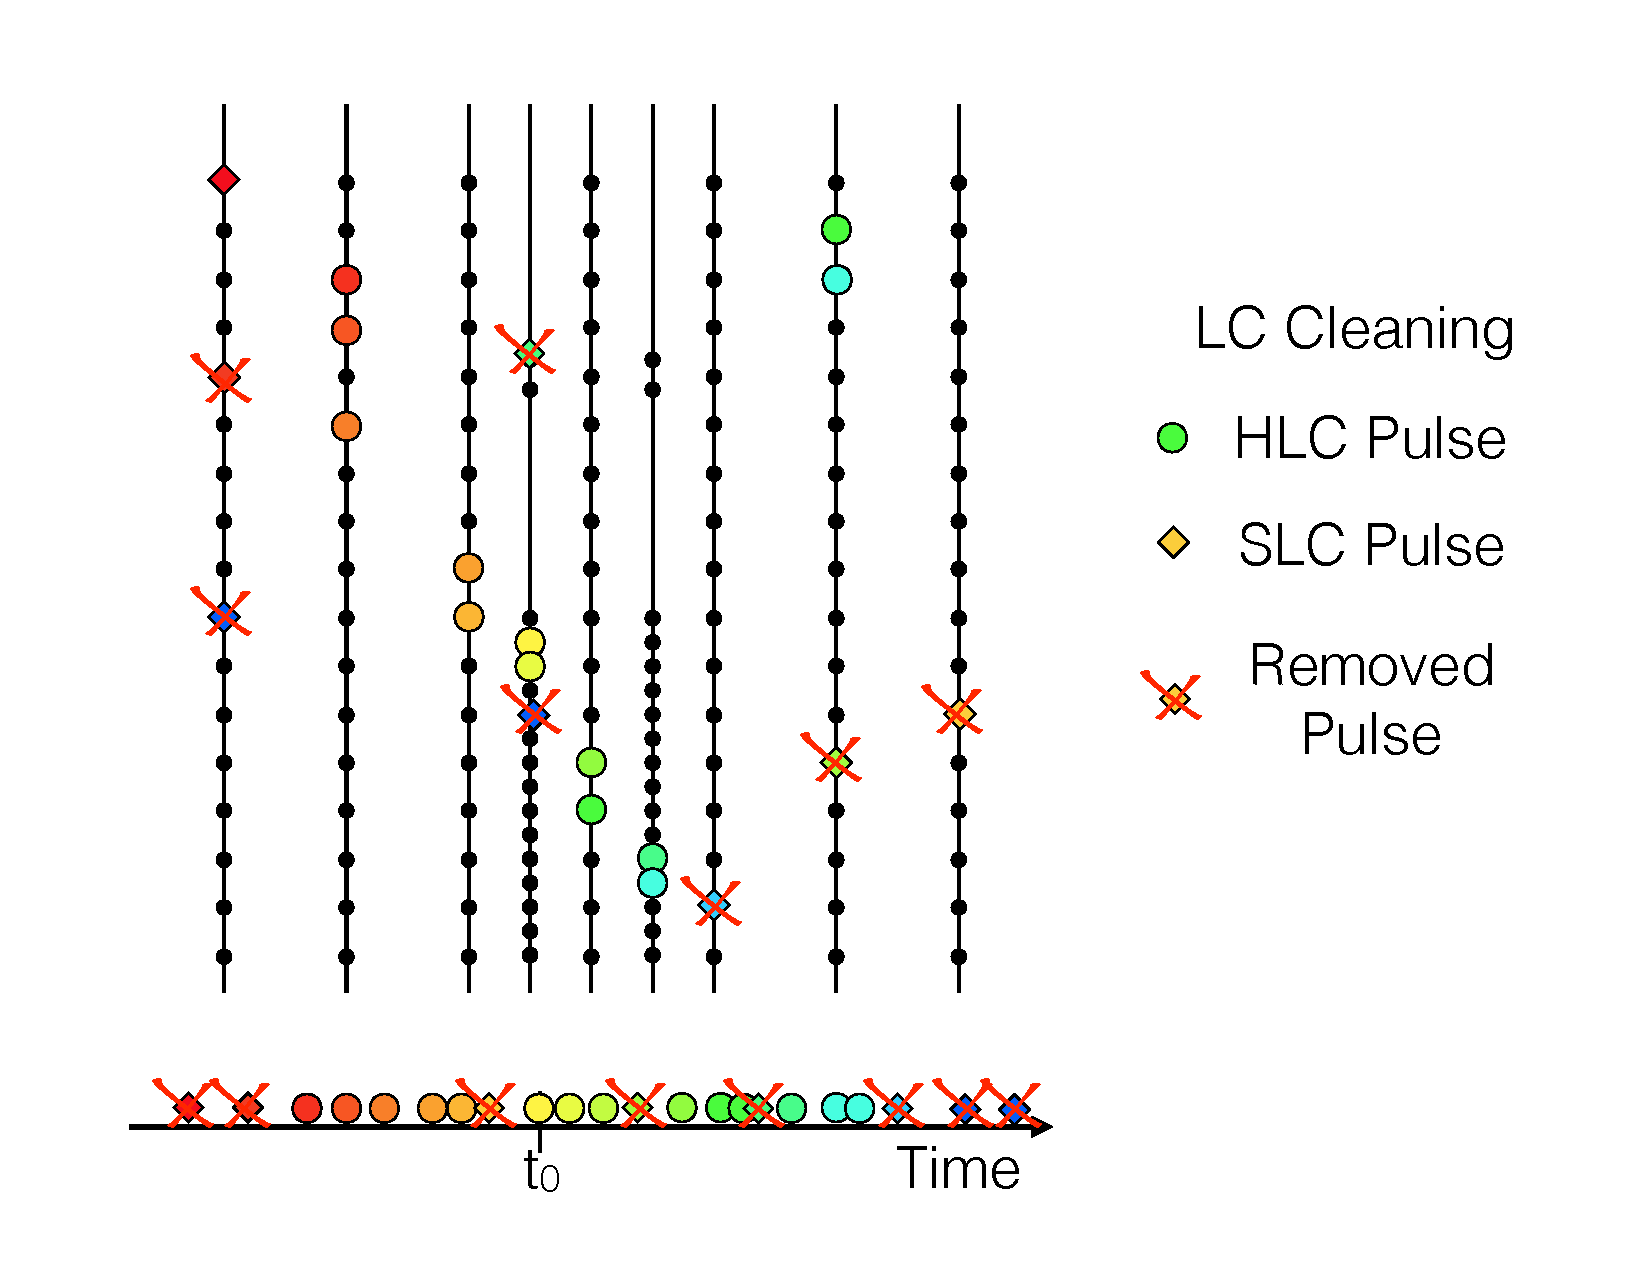
\includegraphics[width=0.3\textwidth]{LCCleaningDiagram.pdf} \\
  \small (\textbf{\color{ctcolormain}a}) HLC Cleaning
\end{tabular} \hspace{2pt}
\begin{tabular}[b]{c}
  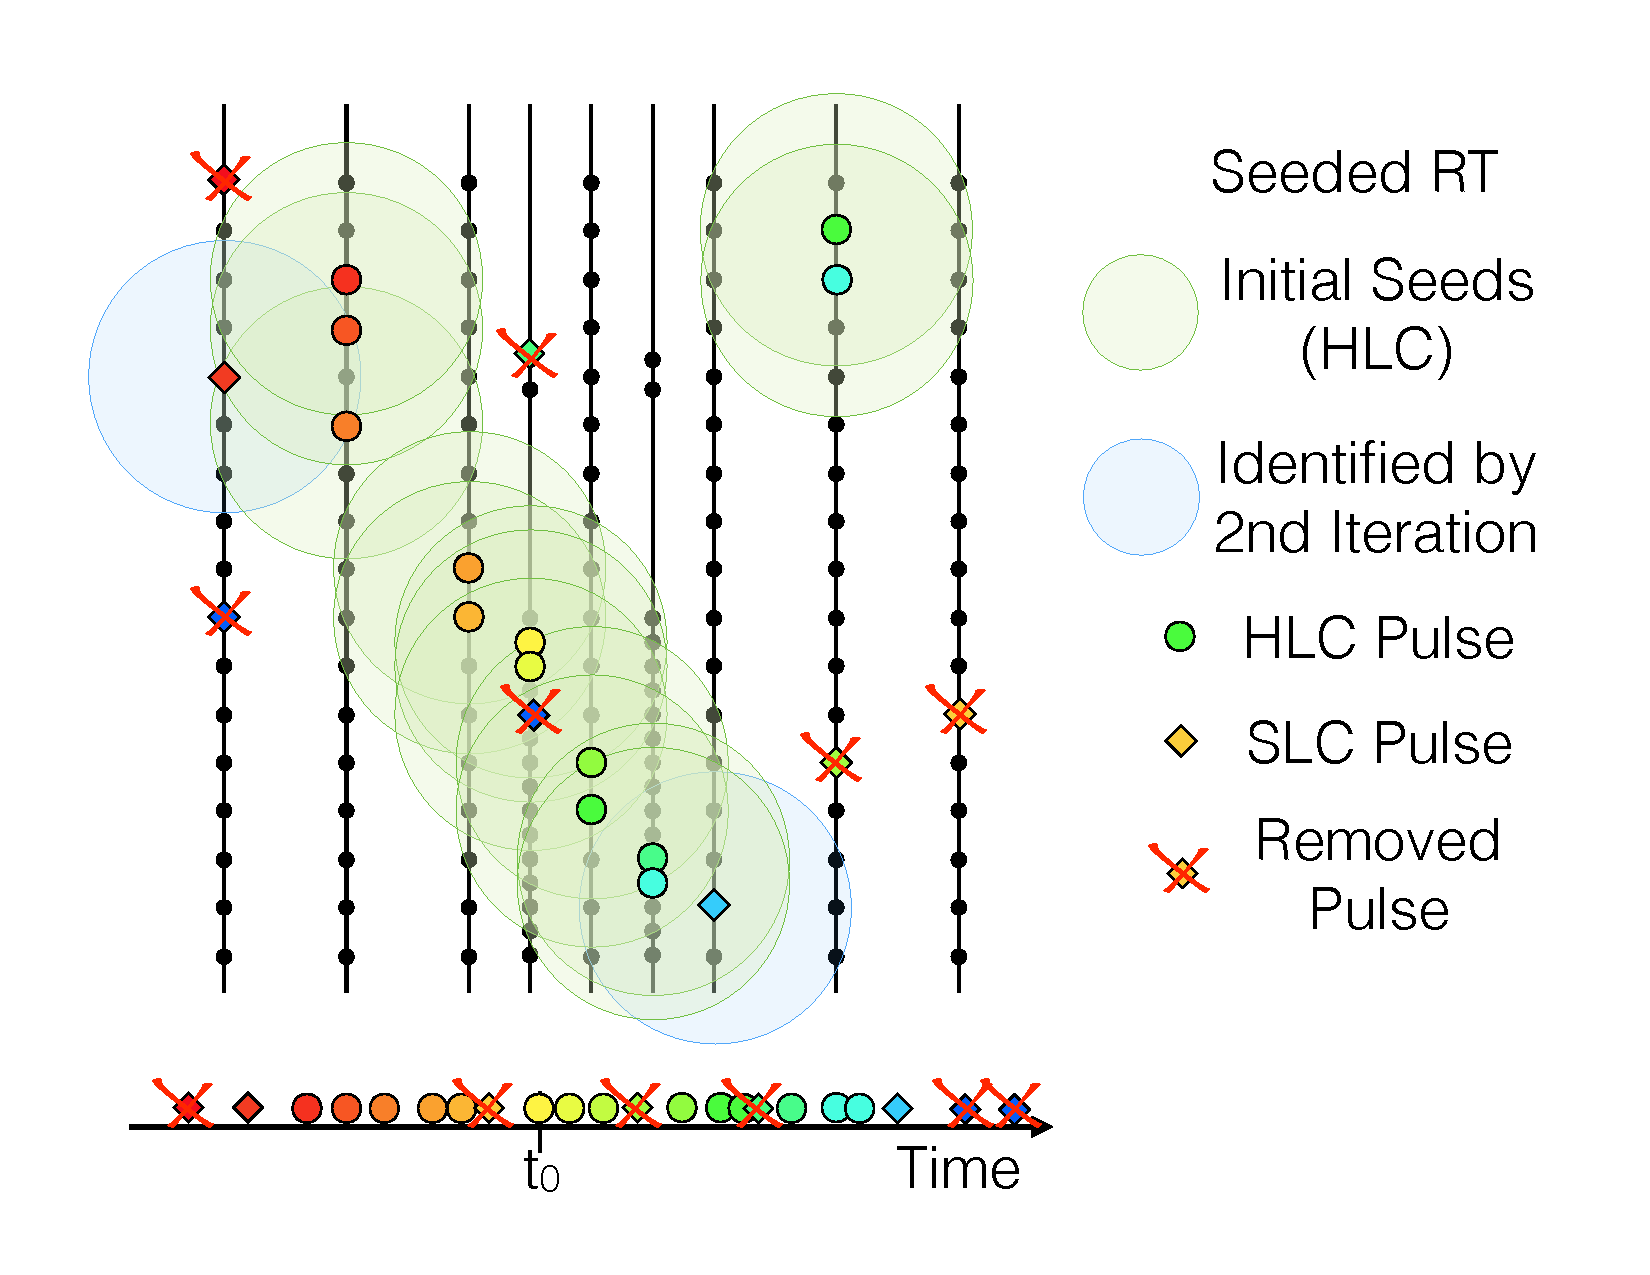
\includegraphics[width=0.3\textwidth]{SRTCleaningDiagram.pdf} \\
  \small (\textbf{\color{ctcolormain}b}) SeededRT Cleaning
\end{tabular}
\begin{tabular}[b]{c}
  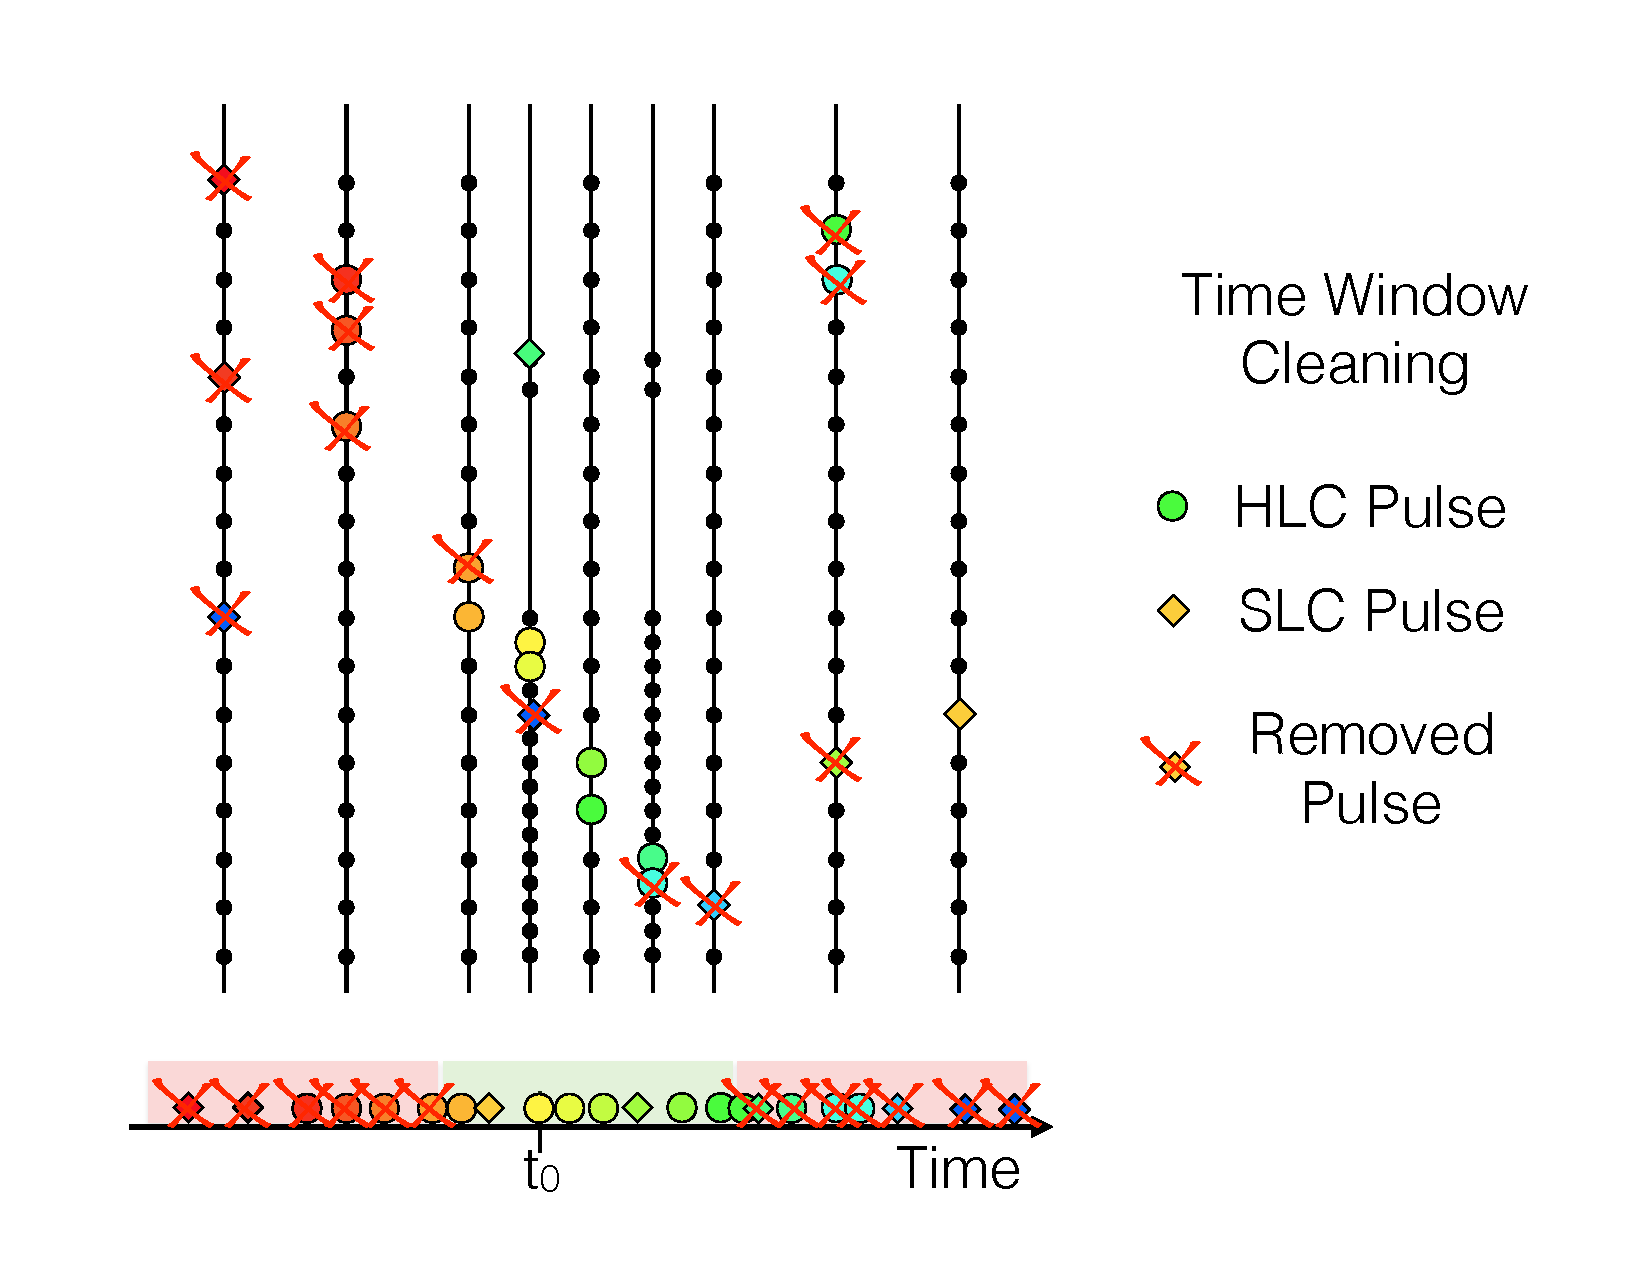
\includegraphics[width=0.3\textwidth]{TWCleaningDiagram.pdf} \\
  \small (\textbf{\color{ctcolormain}b}) Time Window Cleaning
\end{tabular}
\caption[Hit cleaning algorithms in IceCube]{An illustration of the LC, SeededRT, and time window cleaning methods. (Left) All SLC pulses are removed while all HLC pulses are retained. (Middle) Pulses are removed based on time and distance from nearby HLC DOMs, allowing some SLC pulses to be accepted. (Right) Pulses are removed using the time relative to either the trigger in the static time window (STW) cleaning or the maximum pulse density in time in the dynamic time window (DTW) cleaning algorithms. }
\label{fig:hit_cleaning}
\end{figure}

\subsubsection{SeededRT Cleaning}
Instead of using only HLC hits, additional processing may be used to identify potentially interesting SLC pulses as well.
The \emph{SeededRT} (\emph{SRT}) algorithm is one such algorithm, requiring a seed, radius, and time in order to search for additional information in the event as shown in Figure~\ref{fig:hit_cleaning}.
SeededRT begins with a subset of "interesting" pulses, often a selection of the HLC pulses, as a seed.
Once a seed is selected, a sphere is drawn around each seeded DOM. 
Any nearby DOMs observing pulses within the sphere and time window are added to the output pulse series.
Once all seed DOMs have been checked, a new seed is created composed of the all current output pulse series.
The process is repeated until no further pulses are discovered.

The most effective set of parameters is dependent on the detector geometry, since a given radius sphere will contain more DOMs in the DeepCore fiducial than the same sphere outside of DeepCore.
Because of this, different settings are chosen for these two regions.
In the less dense IceCube detector, a radius of 150~m and time window is 1000~ns is used. 
In DeepCore, these values are typically halved, with a raidus of 75~m and a time window of 500~ns.

The SeededRT algorithm is commonly used in IceCube, allowing for a pulse series with minimal noise contributions while finding most hits due to muon or neutrino interactions.

\subsubsection{Time Window Cleaning}
The most permissive pulse cleaning algorithm results in very little loss in pulses due to particle interactions, but allows nearly all noise pulses into the final hit series.
This \emph{Static Time Window} cleaning, often referred to using just the acronym \emph{STW} cleaning, looks for pulses near the time of the trigger.
For DeepCore processing, any pulses more than 4 microseconds before or more than 6 microseconds after the SMT3 time are removed.

There exists a second type of time window cleaning applied more rarely, but used in the GRECO selection.
The \emph{Dynamic Time Window} cleaning, hereafter \emph{DTW} cleaning, is a time window cleaning algorithm that uses the maximum pulse density in time to find a likely interaction time of a muon or neutrino. 
The timing window is placed around this time instead of around the trigger.
DTW cleaning is generally chosen with a significantly tighter window, often consisting of only a few hundred~ns compared to the multiple microseconds used in the STW cleaning.

Time window cleaning is typically used in combination with additional cleaning methods, resulting in little loss in useful signal due to the wide time window (in STW cleaning) or in a very pure set of hits likely to be due to unscattered light.

\section{Level 1: The DeepCoreFilter}
\label{sec:DeepCoreFilter}
Triggers are generally designed to be as accepting of the proposed physics signal as possible within processing contraints.
Typically, limitations exist solely in the processing and storage capabilities.
After triggering, various filters may be applied with the sole purpose of removing the collected background.
For the purposes of this document, the only filter considered is the \emph{DeepCoreFilter}.

The DeepCoreFilter proceeds by splitting the first pulse on each DOM identified by the SeededRT cleaning into "veto" and "fiducial" pulses, with each DOM given a designation based on it's position in the detector as described in Section~\ref{sec:geometry} \cite{Description-DeepCore,Thesis-Vuvuzela}.
All hit DOMs with the first pulse occuring more than one standard deviation away from the mean time are removed from the fiducial pulse series in order to further limit the contributions from noise pulses.

With the updated fiducial pulse series, a center of gravity, or \emph{CoG}, of the remaining hit DOMs is calculated.

\begin{equation}
	\vec{x}_{CoG}=\frac{\sum_i^{Hits} \vec{x}_i}{N_{Hits}}
\end{equation}

The "corrected" average time of the fiducial pulses is then calculated by assuming that the pulse is due to light emission at the CoG, as would be the case for a point-like interaction of a cascade event.
\begin{equation}
	t_{CoG} = \frac{\sum_i^{Hits} t_i^0 - \frac{\left|\left|\vec{x}_i - \vec{x}_{CoG}\right|\right|}{c_{ice}}}{N_{hits}}
\end{equation}
%
where $t_i^0$ denotes the time of the first observed pulse and $\vec{x}$ the position of each DOM.

All veto pulses are then compared to this CoG time and position by calculating an effective particle speed, $v$.

\begin{equation}
v = \frac{\left|\left| \vec{x}_{COG} - \vec{x}_{hit} \right|\right|}{t_{CoG} - t_{hit}}
\end{equation}

\begin{figure}
\centering
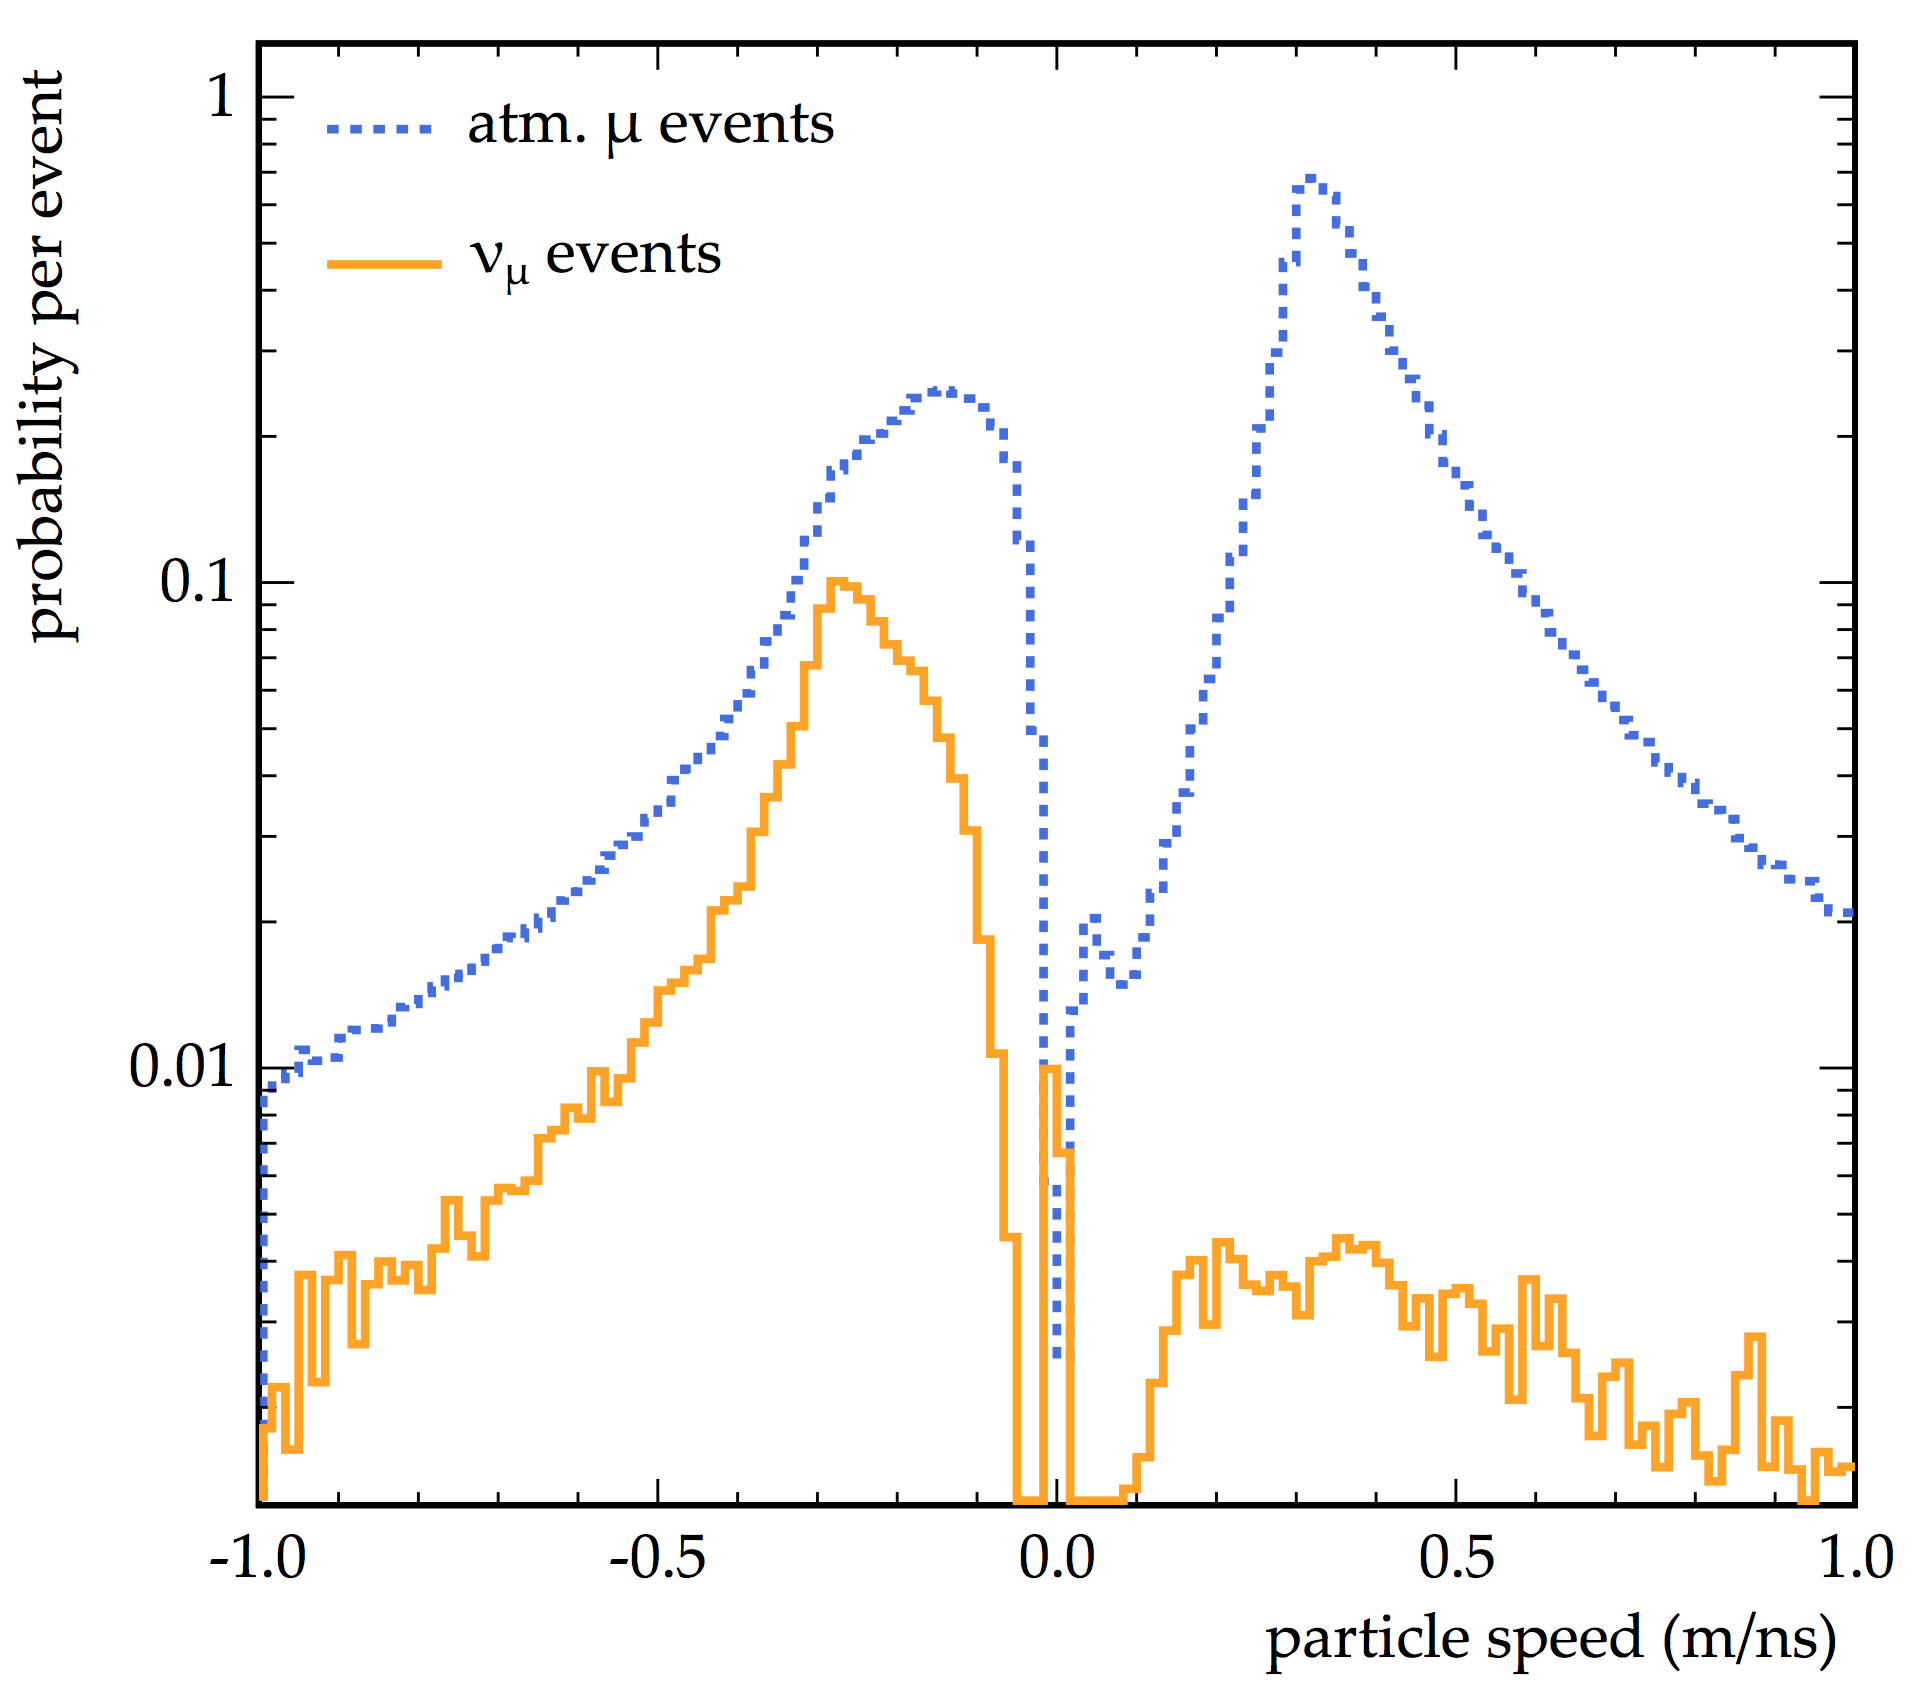
\includegraphics[width=0.7\textwidth]{deepcore_speeds.png}
\caption{The distribution of effective particle speeds used by the DeepCoreFilter to identify and reject muons. Because muons interact first outside of DeepCore, a large peak is visible at speeds around 0.3 m/ns, the speed of light. Figure from \cite{Description-DeepCore}}
\label{fig:deepcore_speeds}
\end{figure}

Muons passing through the detector will do so at the speed of light, 0.3~m/ns. 
Unscattered hits left behind in the detector show this peak clearly for muons as shown in Figure~\ref{fig:deepcore_speeds}.
Low energy neutrino events, on the other hand, typically begin in DeepCore, with hits outside of the fiducial region following hits inside. 
These neutrino events show a peak at negative speeds.
Events with more than one hit with an effective speed $v$ between 0.25~m/ns and 0.4~m/ns are rejected and are removed from further processing.

The DeepCoreFilter is the first step in a low energy analysis in IceCube and is used in many analyses \cite{Thesis-Vuvuzela,Thesis-Euler,IceCube-Oscillation2013,IceCube-Oscillation2015,IceCube-Oscillation2018}.
The algorithm reduces the atmospheric muon background from 280 Hz to approximately 17 Hz while retaining 99.4\% of neutrino events which begin in DeepCore \cite{Description-DeepCore}.

\graphicspath{{chapters/greco/images/Level 3/}}
\section{Low-En Level 3 Cuts}
\label{sec:level3}
After the DeepCoreFilter is used to remove events, variations of hit cleaning algorithms and reconstructions are used.
This processing stage, \emph{Level 2}, does not remove events from the selection and will not be discussed here.

Following the Level 2 processing, the \emph{Low energy Level 3} cuts are introduced.
These cuts are standardized and used in all DeepCore oscillation analyses.
The Level 3 processing follows the same strucure as the following cut levels, cosisting of one set of cuts designed to remove atmospheric muons (\emph{muon rejection} cuts) and another set of cuts selected to remove accidental triggered events (\emph{accidentals rejection} cuts).ß

After the DeepCoreFilter, approximately half of the remaining rate consists of muons.
The remainder is due to accidental triggers due to random detector noise due to the low trigger threshold used in DeepCore.

\subsection{Rejection of Accidental Events at L3}
\label{subsec:level3_noise}
Three cuts are introduced at Level 3 in order to reduce the observed number of accidental triggers.
Events are required to have at least 3 pulses and a total charge of at least 3 PE in a 250~ns DTW cleaned pulse series in the DeepCoreFiducial region.
This removes events which have reached Level 3 processing via random detector noise in the fiducial region.

In addition, the \emph{NoiseEngine} algorithm is used to identify accidental triggers \cite{Thesis-Vuvuzela}.
NoiseEngine uses the relative direction between each pair of hits to search for directionality of the event. 
Events with fewer than three hit pairs pointing in the same direction are rejected.
After the NoiseEngine algorithm, more than 96\% of accidental triggers are removed from the analysis.

\subsection{Rejection of Atmospheric Muon Events at L3}
\label{subsec:level3_muons}
The removal of muons relies on some understanding of the characteristics of these events at Level 3.
Muons at this level are generally bright enough to be identified by hits in the outer part of the detector, known as the veto region.
Because neutrino candidates of interest in this search have energies less than 50 GeV, no light emission is expected in the veto region due to neutrinos.
This may be used to identify muons using cuts described here.

\subsubsection{First Hit Z Position}
Because the muon tracks are primarily steeply inclined, most will leave hits in the upper part of the detector.
Neutrinos of interest in the search for appearance will primarily emit light within the DeepCore fiducial volume, leading to little or no light emission in the top half of the detector. 
This difference between neutrino and muon emission veto region is used to identify background muons
The position of the first hit in a STW+SRT cleaned pulse series consisting of DeepCore fiducial hits is used to look for muons using this principle.
Any event with a first hit above Z=-120~m is removed.

\subsubsection{NAbove200}
The total charge of recorded hits occuring in the top of the detector is also used in the analysis. 
This variable, known as \emph{NAbove200}, measure the integrated charge occuring before the SMT3 trigger above a depth of -200	.
If more than 12 DOMs are hit above Z=-200 m, then the event is removed.

\subsubsection{RTVeto}
The SeededRT algorithm is useful for removing noise hits in the detector.
It may also be used to find clusters of hits due to muons in the outer part of the detector as well.
This technique, known as \emph{RTVeto}, uses the SeededRT algorithm to identify the largest cluster of pulses in the veto region.
The number of hits in this cluster is used to identify atmospheric muon events.
The RTVeto algorithm uses a radius of 250~m and a time window of 1000~ns for both DeepCore and IceCube DOMs.

The cut is used in combination with the total amount of charge observed in the DeepCore fiducial region to define a few separate cut conditions.
For the purposes of this search, only the lowest energy version is relevent.
In this case, any event with a cluster of 4 or more hit DOMs in the outer detector is removed.

\subsubsection{C2QR6}
Atmospheric muon events at Level 3 tend to leave long tracks and take O(3 $\mu$s) to cross the detector.
Oscillation neutrino events prouce small light patterns due to the low energies involved, with light being deposited quickly.
The difference in the light emission profile of the two event types may also be exploited to reject atmospheric muons background events.

To evaluate the deposition time for light in each event, the \emph{charge ratio in 600 ns} (\emph{QR6}) is used.
QR6 is defined as the ratio of charge observed in the first 600~ns and the total amount of observed charge.

\begin{equation}
QR6 = \left.\frac{\sum_i q_i}{\sum_i^{hits} q_i}\  \right\rvert_{0~\leq~t_i-t_{first}~<~600}
\end{equation}

Here the time is measured relative to the first observed hit in a STW+SRT pulse series.
Atmospheric muons will tend to deposit light over a longer timescale, resulting in a charge ratio near 0.
Neutrinos will deposit light quickly, with a charge ratio near 1.

The algorithm is sensitive to the first observed hit.
Noise hits before the particle interaction can lead to an erroneous definition of the time window.
In order to reduce this possibility, the first two hits may be ignored for the calculation. 
This form, the \emph{cleaned charge ratio in 600 ns} (\emph{C2QR6}) is used in the Level 3 processing to remove atmospheric muon events.

\subsection{Rates at Level 3}
\begin{table}[]
\centering
\begin{tabular}{@{}llll@{}}
\toprule
\multirow{2}{*}{Type} & \multicolumn{3}{c}{IceCube Processing} \\
                      & Any Filter   & DC Filter  & Low-en L3  \\ \midrule
CORSIKA               & 990598       & 9178       & 969.818    \\
MuonGun               & 60669        & 2982       & 442.493    \\
Accidentals           & 35855        & 8117       & 283.559    \\
$\nu_e$               & 1.842        & 1.721      & 1.262      \\
$\nu_{\mu}$           & 11.317       & 6.360      & 4.758      \\
$\nu_{\tau}$          & 0.293        & 0.270      & 0.206      \\ \midrule
MC Total*             & 1026466      & 17303      & 1260       \\
Data                  & 1154426      & 19092      & 1092       \\ \bottomrule
\end{tabular}
\caption{The event rates after the Level 3 cuts in GRECO. The total simulated rate is calculated using CORSIKA events and ignoring MuonGun. The data is estimated from a burn sample of 14 days. Rates are given in mHz.}
\label{tab:event_rates_L3}
\end{table}

The rates after the Level 3 cuts are applied are shown in Table~\ref{tab:event_rates_L3}. 
The atmospheric muons are reduced by about an order of magnitude.
The removal of accidental triggered events forms a large part of the reduction in rate at Level 3, with the rates decreased by more than 96\%.


\graphicspath{{chapters/greco/images/level4/}}
\section{GRECO Level 4 Cuts}
\label{sec:level4}
The first GRECO-specific cut level is designated \emph{Level 4}, or \emph{L4} and was first introduced in 2011 using very similar variables as the Level 3 cuts.
This is performed for historical reasons, as the DeepCore Level 3 and GRECO Level 4 were produced in parallel.

As in the DeepCore Level 3 processing, the GRECO Level 4 is divided into two types of cuts: those that remove accidental triggers due to detector noise and those that remove atmospheric muons. 
The cuts for atmospheric muons are fed into a \emph{boosted decision tree} (\emph{BDT}), a multivariate algorithm designed to separate signal from background \cite{TMVA}.
 
\subsection{Rejection of Accidental Events at L4}
Similar to the cuts applied at Level 3, the GRECO Level 4 begins with a cut on the number of observed hits. 
In this case, static time window cleaning is applied with a range of $-3500~ns \leq t \leq 4000~ns$ for hits in the DeepCore fiducial volume.
A dynamic time window cleaning is then applied with a window of 200 ns.
Any events with fewer than three hits in this stricter pulse series is removed.

\subsection{Rejection of Atmospheric Muon Events at L4}
Some cuts used to identify muons in the GRECO Level 4 are similar to those applied in the Level 3 processing. 
A stricter hit cleaning algorithm is used at this cut level to identify muons missed at Level 3.
The reprocessed cuts are then used to train a \emph{boosted decision tree} (\emph{BDT}).

\subsubsection{FirstHit Z}
\begin{figure}[h]
	\centering
		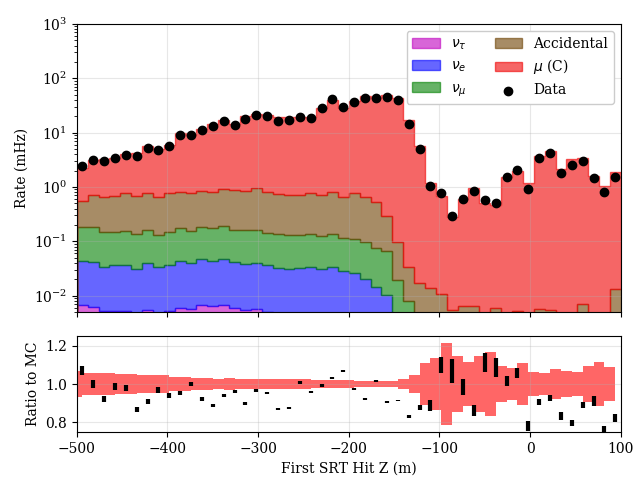
\includegraphics[width=0.45\linewidth]{FirstHitZ_log.png}
		\caption[The FirstHit Z position]{The Z position of the first hit in a cleaned hit series. Note the shape difference between the atmospheric muons in red and the various neutrino flavors, particularly above -200~m.}
	\label{fig:firsthitz_log}
\end{figure}

The Z position of the first hit DOM in the event is included for the GRECO Level 4. 
The cut continues to show separation between neutrino events and atmospheric muons with the new hit cleaning.

\subsubsection{NAbove200}
\begin{figure}[h]
	\centering
		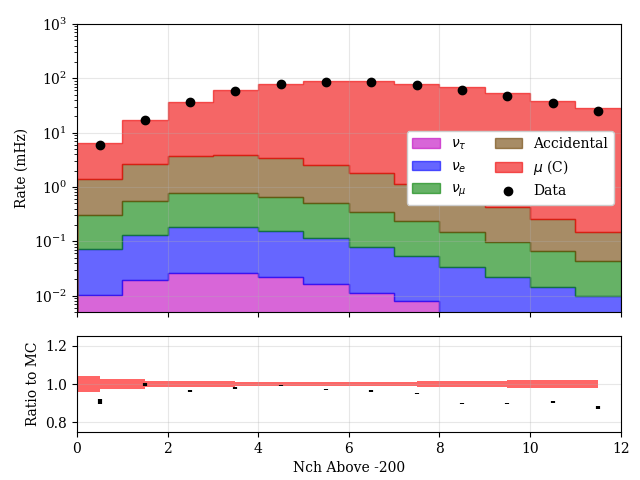
\includegraphics[width=0.45\linewidth]{NAbove200_log.png}
		\caption[Number of Hits Above Z=-200]{The number of hits above Z=-200~m}
	\label{fig:nabove200_log}
\end{figure}

Similarly, the number of hit DOMs identified above Z=-200~m is again used with a new hit series.
Once again, some separating power remains.

\subsubsection{QR6/C2QR6}
\begin{figure}[h]
\centering
\begin{tabular}[b]{c}
  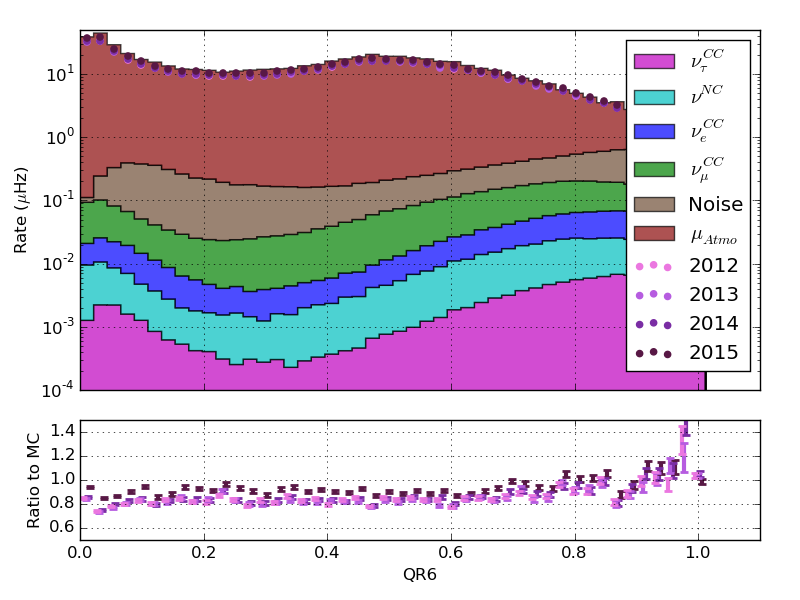
\includegraphics[width=0.45\linewidth]{QR6_log.png} \\
  \small (\textbf{\color{ctcolormain}a}) QR6
\end{tabular} \hspace{2pt}
\begin{tabular}[b]{c}
  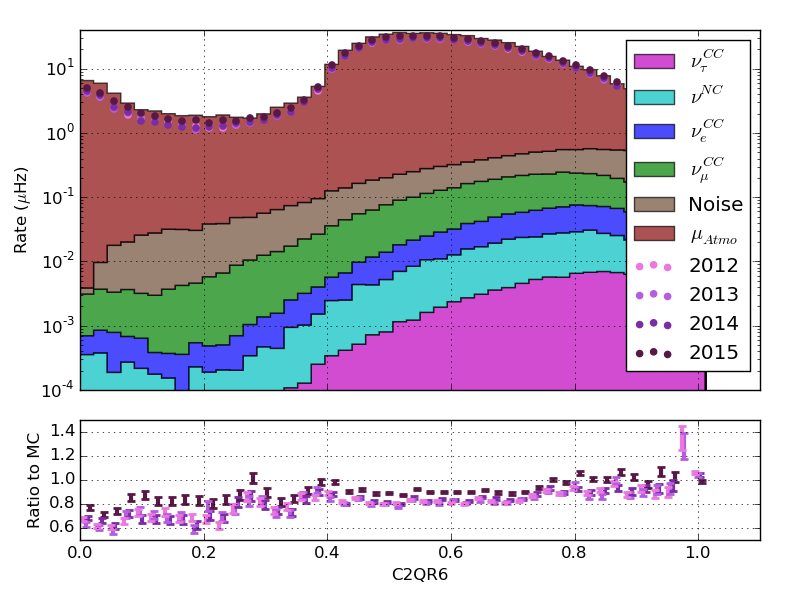
\includegraphics[width=0.45\linewidth]{C2QR6_log.png} \\
  \small (\textbf{\color{ctcolormain}b}) C2QR6
\end{tabular}
\caption[QR6 and C2QR6]{The charge ratio variables used in the GRECO Level 4 cuts.}%
\label{fig:QR6_and_C2QR6}%
\end{figure}

Both the QR6 and C2QR6 are used in the GRECO Level 4 processing. 
The two show some degeneracy, although the BDT shows weaker separation if only one is available.
Note that there exists some significant disagreement between data and simulation at low values of C2QR6.
This region does not contain much signal and will be removed by the BDT.

\subsubsection{Tensor of Inertia}
\begin{figure}[h]
	\centering
		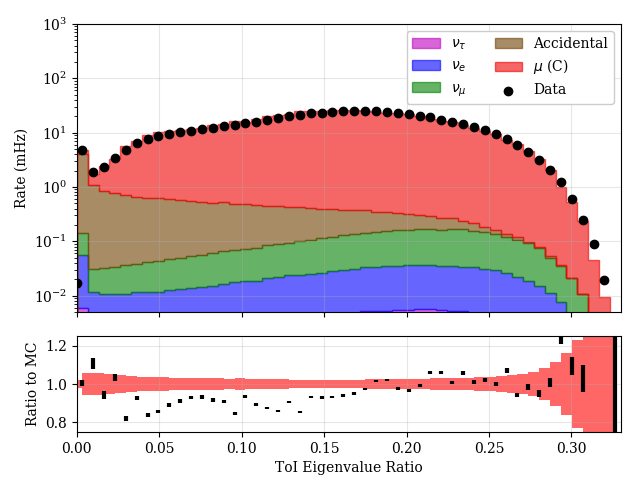
\includegraphics[width=0.45\linewidth]{ToIEval_log.png}
		\caption[Tensor-of-Inertia Eigenvalue Ratio]{The eigenvalue ratio from a ToI calculation. Larger values indicate more apparent elongation in the event.}
	\label{fig:toi_log}
\end{figure}

At early cut levels, the muon and neutrino hit patterns appear different spatially in the detector.
Many neutrinos with energies in the range of 1-100~GeV will have a compact hit pattern in DeepCore.
Muons will have a more elongated hit pattern.
The different hit topologies may be measured with the \emph{Tensor of Inertia eigenvalue ratio} (more briefly, \emph{ToI}).
This variable is defined in analogously to the tensor of inertia from mechanics, with the measured charge taking the place of the mass.

\begin{equation}
\begin{tabular}{c}
	I_{X} = \sum_{i=0}^{nhits}(y_i^2 + z_i^2)q_i	\\ \\
	I_{Y} = \sum_{i=0}^{nhits}(x_i^2 + z_i^2)q_i \\ \\
	I_{Z} = \sum_{i=0}^{nhits}(x_i^2 + y_i^2)q_i \\
\end{tabular}
\end{equation}

These three moments yield information about the shape of the event.
The eigenvalue ratio is defined as 

\begin{equation}
	e = \frac{{max}(I_j)}{I_{x}+I_{y}+I_{z}}
\end{equation}

Events which are very track-like, and therefore muon-like, have eigenvalue ratios near 0 while more cascade-like events have eigenvalue ratios close to $\frac{1}{3}$.


\subsubsection{Linefit Speed}
\begin{figure}[h]
	\centering
		\includegraphics[width=0.45\linewidth]{iLineFit_Log.png}
		\caption[The improvedLineFit Speed]{The effective speed of a plane wave passing through the detector measured in~m per nanosecond.  Faster speeds are associated with atmospheric muons traveling in ice at speeds $c$. Neutrino events below 50 GeV appear more isotropic, with effective speeds close to 0.}
	\label{fig:ilinefit_log}
\end{figure}

\emph{LineFit} is an first-guess reconstruction used in IceCube.
The algorithm fits the hits in the detector with a plane wave moving at speed $\vec{v_{LF}}$.
The speed of the plane wave may be solved analytically \cite{LineFit}.

\begin{equation}
\vec{v}_{LF} = \frac{\left<t_i \cdot \vec{x}_i \right> - \left<\vec{x}_i\right>\left<t_i\right>}{\left<t_i^2\right> - \left<t_i\right>^2}
\end{equation}
%
where $\left<t_i\right>$ denotes the average hit time and $\vec{x}_i$ is the average hit position in the detector.
In cascade-like events, photons have no average preferred direction, resulting in an average velocity close to 0.
The relativistic atmospheric muons do have a preferred direction and travel through the detector with speed $c_{ice}$~=~0.3~m/ns.

\subsubsection{The L4 BDT}
\begin{figure}[h]
	\centering
		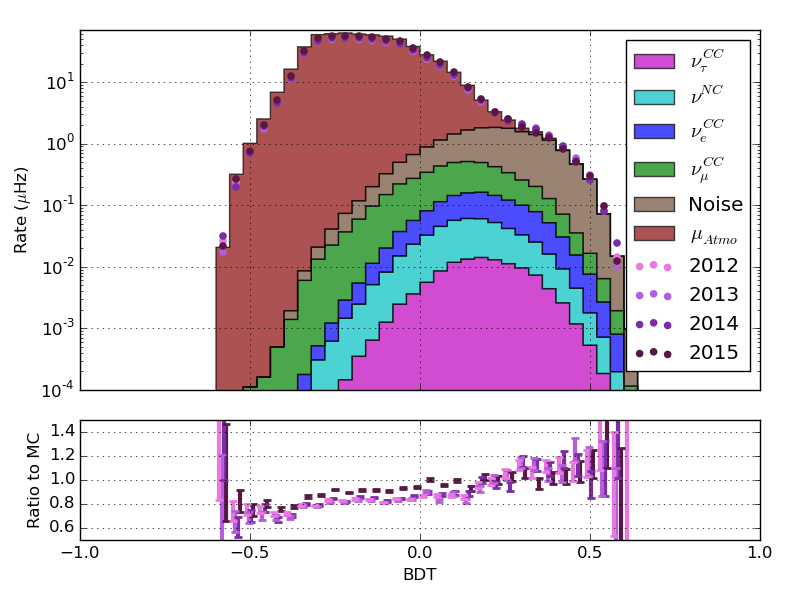
\includegraphics[width=0.9\linewidth]{BDT_log.png}
		\caption[The L4 BDT Score]{The distribution of the boosted decision tree decision score used at L4. A cut is applied at 0.04 to remove a significant fraction of atmospheric muon background events. Note the ratio, which shows disagreement in the very muon-like region. The region of disagreement is removed by the cut.}
	\label{fig:L4_bdt_log}
\end{figure}

A Boosted Decision Tree (\emph{BDT}) is trained at L4 to further reduce the atmospheric muon background by a factor of 10x. 
The variables described above were provided to a BDT training using CORSIKA muon simulation as the background training sample and GENIE simulation as the signal sample. 
The BDT uses a series of \emph{trees}, collections of multidimensional cuts, to classify events as either signal-like or background-like \cite{TMVA}.
After \emph{boosting}, a process by which event weights are adjusted based on the success or failure of previous classification attempts, the BDT returns a \emph{score} ranging from -1 (background-like) to +1 (signal-like) which may be used as a cut variable in an analysis.

The scores returned by the GRECO Level 4 BDT are shown in Figure~\ref{fig:L4_bdt_log}.
The distribution ranges from -0.6 to +0.6, indicating that no signal or background events are perfectly identifiable.
Separation is observed between the atmospheric muon events, which peak around a score of -0.25, and signal, peaking at +0.15.

Comparisons to MC show mild disagreement between data and Monte Carlo, particularly in the most muon-like regions that get cut away. 
Its not obvious what causes the disagreement, although it is possible that the cosmic ray flux model is simply an inaccurate model of some part of the spectrum. 
Alternatively, this may be an artifact of undiscovered mismodeling of the atmospheric muon events.
High energy muon events would likely have clear tracks visible in the detector, contributing to the region around -0.5.
If the flux or simulation of these events does not reflect data, the BDT score distribution would be expected to show the largest disagreement in the background dominated region below -0.2.
No investigation of the disagreement has been performed, as these events are removed from the GRECO selection.

A shoulder attributable to the accidental triggers is visible at high values of the BDT score, peaking around 0.25, indicating that these events appear more signal-like than the nuetrino samples.
While initially puzzling, investigation of the training of the BDT showed that the original training sample did not include accidental triggered events.
Instead, only CORSIKA and GENIE events were used to train the BDT.
Because the training lacked any accidental triggers, the BDT picked the most obvious feature of the GENIE sets: that the signal events were primarily low energy with lower light deposition than the background muons. 
These are also key features of the noise triggers. 

The GRECO Level 4 places a cut at 0.04 in the BDT score, removing a large fraction of the background sample.
A large fraction of the neutrino sample is also removed in order to reduce the muon rates by a factor of 20x.

\subsection{Rates at Level 4}
\begin{table}[]
\centering
\begin{tabular}{@{}lllll@{}}
\toprule
Type         & \multicolumn{3}{c}{IceCube Processing} & GRECO  \\
             & Any Filter   & DC Filter  & Low-en L3  & L4     \\ \midrule
CORSIKA      & 990598       & 9178       & 969.818    & 50.511 \\
MuonGun      & 60669        & 2982       & 442.493    & 33.562 \\
Accidentals  & 35855        & 8117       & 283.559    & 11.963 \\
$\nu_e$      & 1.842        & 1.721      & 1.262      & 0.783  \\
$\nu_{\mu}$  & 11.317       & 6.360      & 4.758      & 2.503  \\
$\nu_{\tau}$ & 0.293        & 0.270      & 0.206      & 0.134  \\ \midrule
MC Total*    & 1026466      & 17303      & 1260       & 65.893 \\
Data         & 1154426      & 19092      & 1092       & 68.592 \\ \bottomrule
\end{tabular}
\caption{The event rates after the Level 4 cuts in GRECO.  The total simulated rate is calculated using CORSIKA events and ignoring MuonGun. The data rate is estimated from a burn sample of 14 days. Rates are given in mHz.}
\label{tab:event_rates_L4}
\end{table}

The rates of the selection after the Level 4 cuts are applied are shown in Table~\ref{tab:event_rates_L4}.
After the GRECO Level 4 BDT, the number of atmospheric muons is reduced to 50 Hz, a mere 25x the muon neutrino rate.
The number of accidental triggers is also reduced in the analysis due to the dedicated cuts applied at this level.
The number of accidental triggers is still larger than the number of neutrinos expected, however, indicating that further cuts are necessary.












\graphicspath{{chapters/greco/images/level5/}}
\section{GRECO Level 5 Cuts}
\label{sec:level5}
The next stage of cuts, know as the \emph{GRECO Level 5}, or more simply, \emph{L5}, also uses a BDT to remove atmospheric muon background events.

\subsection{Rejection of Accidental Events at L5}
Unlike the previous stages, there is no explicit cut introduced at L5 to remove accidental triggers.
Instead, an implicit requirement on the number of hit DOMs arises due to the reconstruction used at Level 5.

The STW+SRT pulse series containing DeepCore fiducial pulses is used to fit a total of 6 free parameters: the position (x, y, z), the time (t), and the direction of a muon track (zenith, azimuth).
The parameters are degenerate if fewer than five hits are used.
In this case, the reconstruction fails to converge and the event is removed.
Because of this degeneracy, the GRECO Level 5 requires at least 6 hit DOMs in the hit series.

\subsection{Rejection of Atmospheric Muon Events at L5}

\subsubsection{Time to 75\% Charge}
\begin{figure}[h]
	\centering
		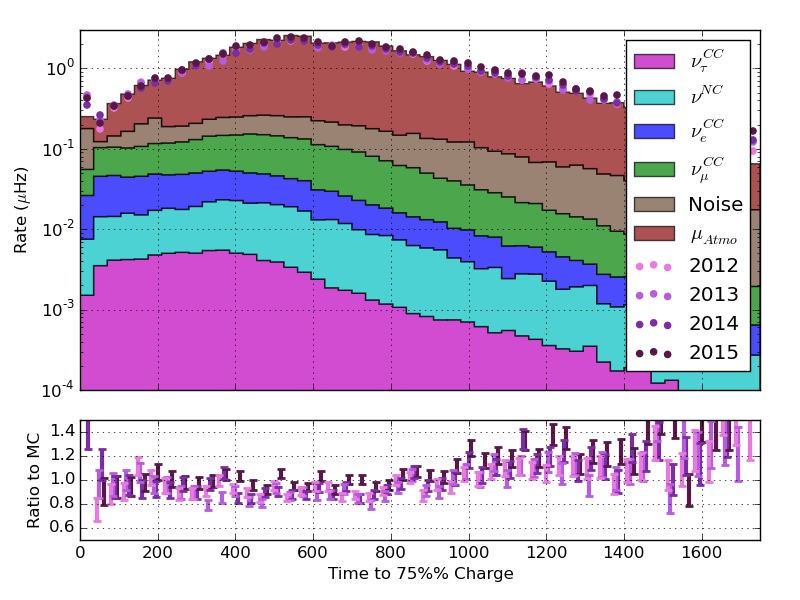
\includegraphics[width=0.45\linewidth]{Time_to_75_Charge_log.png}
		\caption[Time to 75\% Charge]{The time to accumulate 75\% of the total charge of the event. Atmospheric muons tend to produce light in the detector over a longer time than the low energy atmospheric neutrinos used in the search for tau neutrino appearance.}
	\label{fig:time_to_75}
\end{figure}

The first variable used to create the L5 BDT is the amount of time required to record 75\% of the total charge, the \emph{$t_{75}$}, measured from the start of the event.
Similar to the QR6 and C2QR6 variables, the $t_{75}$ is a variable designed to look at the hit distribution in time.
However, the variable is now produced in the reverse manner: where the QR6 variable refers to the amount of charge in a given window, the $t_{75}$ instead attempts to find the amount of time for a given charge level.
Figure~\ref{fig:time_to_75} shows the distribution of the $t_{75}$.

The neutrino events deposit energy quickly due to the low energies of the sample of interest in this thesis.
The muon events take longer to reach 75\% of the total charge due to the long travel time of the muons through the detector.

\subsubsection{Veto Identified Causal Hits}

\begin{figure}[h]
\centering
  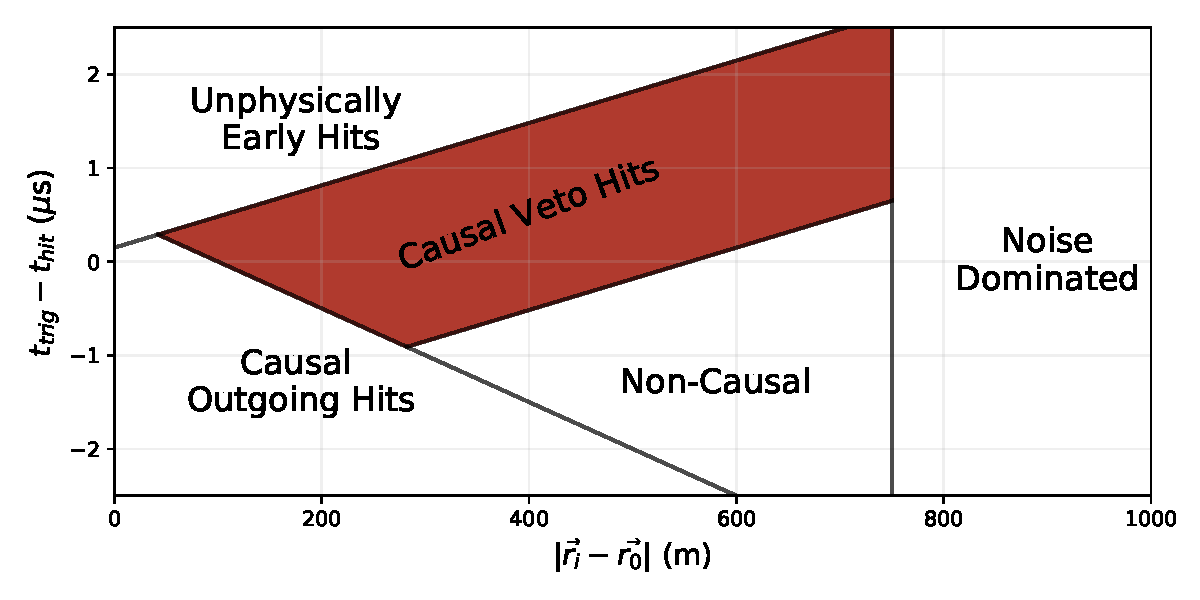
\includegraphics[width=0.7\linewidth]{vich_diagram.pdf} \\
\caption{A schematic diagram showing the regions of the VICH algorithm. VICH returns the number of hit DOMs in the shaded region, corresponding to the pulses that are both causally connected with the trigger and entering DeepCore. }
\label{fig:vich_diagram}
\end{figure}

\begin{figure}[h]
	\centering
		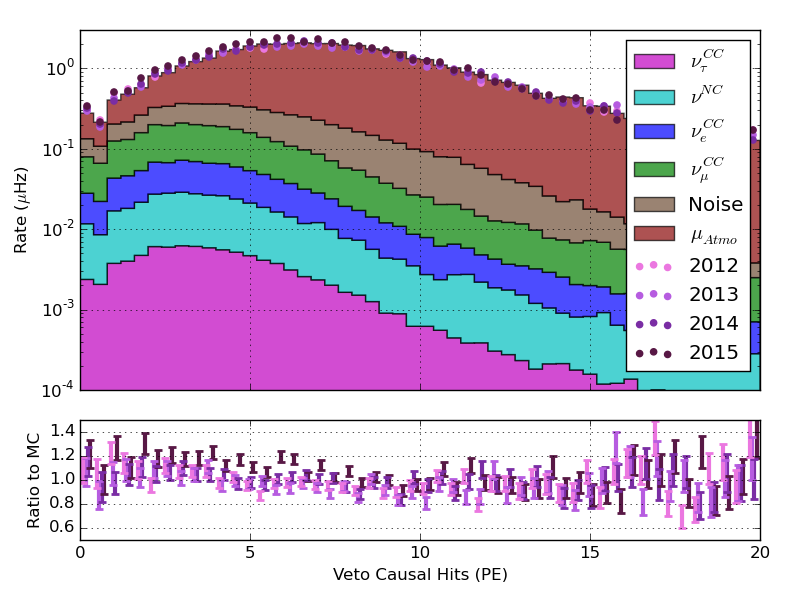
\includegraphics[width=0.45\linewidth]{Veto_Causal_Hits_(PE)_log.png}
		\caption[Veto Identified Causal Hits]{The amount of causally-connected charge discovered in the veto region.}
	\label{fig:vich}
\end{figure}

The \emph{Veto Identified Causal Hits} (\emph{VICH}) algorithm is also used in the GRECO Level 5.
This algorithm uses an uncleaned pulse series to search for hits that are causally connected to the trigger \cite{Thesis-Euler}.
The first DOM to contribute to the DeepCore trigger is used to define the trigger time and position.

Five regions are defined based on the causality criteria shown in Figure~\ref{fig:vich_diagram}.
Hits which are not causally connected to the trigger are ignored. 
Hits which occur too far away from DeepCore are also ignored to reduce the effect of detector noise.
A causal region which is consistent with light travel outgoing from the trigger position is also ignored.

The VICH algorithm returns the total integrated charge of all pulses in the remaining "causal veto region".

\subsubsection{First Hit $\rho$}
\begin{figure}[h]
	\centering
		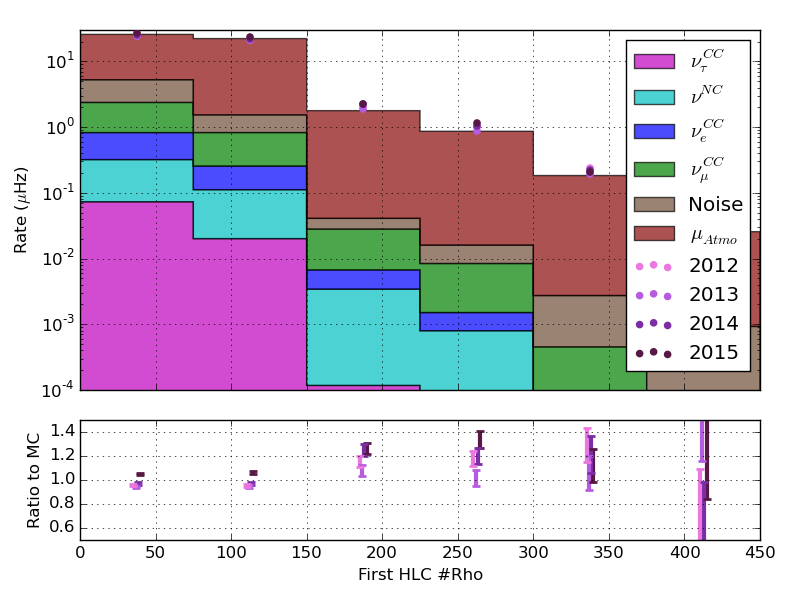
\includegraphics[width=0.45\linewidth]{First_HLC_Rho_log.png}
		\caption[First Hit $\rho$ Position]{The radial position of the earliest hit of a cleaned hit series. The radial position is measured relative to string 36, the center of DeepCore.}
	\label{fig:firsthit_rho}
\end{figure}

The Z position of the first hit was used in the GRECO Level 4 cuts in order to indentify atmospheric muons coming from above DeepCore.
The X and Y position may also be used to identify muons.
These are combined to define a \emph{radial distance} (\emph{$\rho_{36}$}) from the center of DeepCore, here defined to be the position of string 36 at $(x_0,y_0)=(46.3~m, -34.9~m)$.

\begin{equation}
\rho_{36} = \sqrt{\left(x-x_0\right)^2 + \left(y-y_0\right)^2}
\end{equation}

The radial distance is a general parameter and can be used with any event vertex estimator. 
For the GRECO Level 5, the first hit in the STW+SRT pulse series is used.
Atmospheric muons entering DeepCore are more likely to be found at larger values of $\rho_{36}$ while neutrinos are more likely to be found within the DeepCore fiducial volume, which stops at $\rho_{36}=125$~m.

\subsubsection{Quartiles CoG}
\begin{figure}[h]
	\centering
		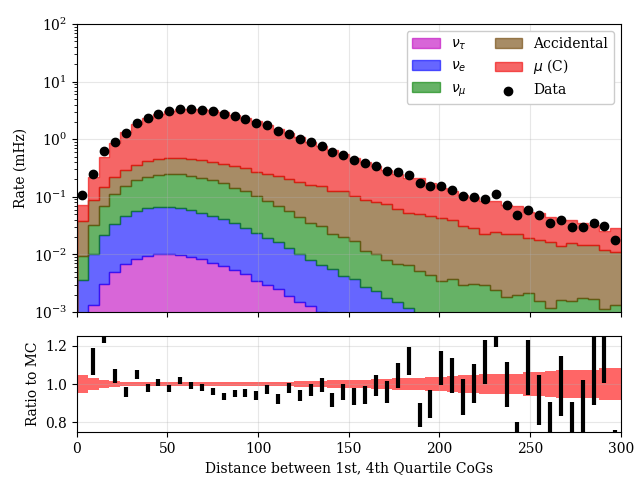
\includegraphics[width=0.45\linewidth]{Q1-Q4_Distance_log.png}
		\caption[Quartile Distance]{The distance between the centers of gravity of the first and last quartile in time.}
	\label{fig:quartile_distance}
\end{figure}

Atmospheric muons at GRECO Level 5 travel through the detector, leaving an elongated track-like hit pattern.
Neutrinos below 100 GeV travel much smaller distances.
The apparent distance traveled by a particle is therefore a useful measure of the particle type.
In GRECO Level 5, the distance between the CoGs of the first and last quartiles in time are used to characterize the distance traveled by the interacting particle.
For atmospheric muon events, this distance is expected to be larger than for low energy neutrino events.

\subsubsection{Z-Travel}
\begin{figure}[h]
	\centering
		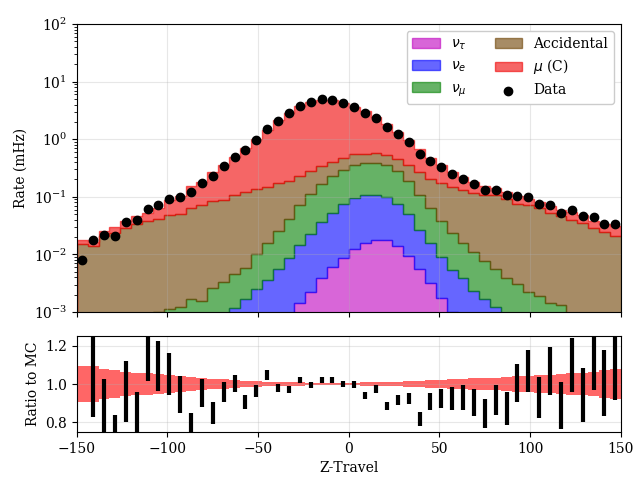
\includegraphics[width=0.45\linewidth]{Z-Travel_log.png}
		\caption[Quartile Z-Travel]{The distance traveled in Z between the first and last quartile of hits in time.}
	\label{fig:quartile_ztravel}
\end{figure}

Because atmospheric muons cannot penetrate the Earth, no background muon events are upgoing.
The distance and direction of travel in the Z coordinate can be a useful variable to identify atmospheric muon events.
The value, known as the \emph{z-travel}, uses the CoG of the first quartile of hits in time as a starting vertex.
Z-travel is the charge weighted average distance in the Z direction of pulses from this vertex

\begin{equation}
\Delta Z = \frac{\sum_i^{pulses} q_i \left(z_i - z_{CoG}\right)}{\sum_i^{pulses}q_i}
\end{equation}

Atmospheric muons traveling through the detector from above will have a negative z-travel distance and neutrinos may be positive or negative, but is likely to be small due to the small size of neutrino events.

The accidental triggers also are also well-separated from the simulated neutrinos.
In the accidental triggers, pulses occur randomly throughout the detector.
These events do not have a preferred direction and appear at all values of the z-travel.
The accidental events dominate at the tails of the distribution.

\subsubsection{SPE Zenith}
\begin{figure}[h]
	\centering
		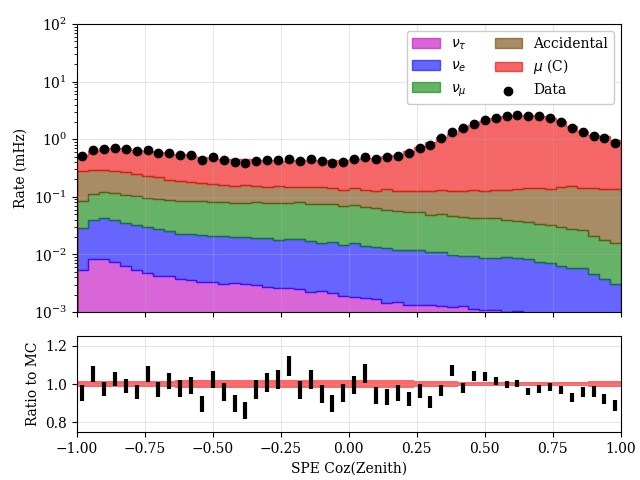
\includegraphics[width=0.45\linewidth]{SPE11_Cos(Zenith)_log.png}
		\caption[SPE Reconstruction Zenith Angles]{The zenith angle distribution of events from an 11-iteration SPE fit. The fit assumes an infinite track hypothesis and uses only hit DOMs.}
	\label{fig:spe11_zenith}
\end{figure}

Previous cut levels used the first HLC hit position or various CoG calculations as analytic estimates the properties of particles in each event.
These estimators are fast and computationally inexpensive to run on large samples of atmospheric muon background events.
At Level 5, the rates are low enough that a \emph{likelihood reconstruction} can be run on the sample, offering additional information about particles in each event.

The \emph{SPE reconstruction} is the first likelihood reconstruction used in the GRECO event selection.
This reconstruction includes a model of the effect of scattering in the ice based on the time of the first observed pulse in each DOM.

The minimum time required for a Cherenkov photon to reach a DOM from an emission point is 

\begin{equation}
t_{point} = t_{emission} + \frac{n}{c} \left|\vec{r}\right| 
\end{equation}
%
where $\left|\vec{r}\right|$ is the distance between the emission point and the DOM.
The corresponding time from a muon track is 

\begin{equation}
t_{track} = t_{emission} + \frac{\vec{r} \cdot \hat{n} + \rho \tan \theta_C}{c}
\end{equation}
%
where $\hat{n}$ is a unit vector pointing in the direction of the muon track, $\theta_C$ is the Cherenkov angle, and $\rho = \left|\vec{r} - \left(\vec{r} \cdot \hat{n}\right) \hat{n}\right|$ is the impact parameter of the track with respect to the DOM \cite{Thesis-Jakob}.
In the absence of scattering, all photons would arrive at the DOM according to these formulae.
The addition of scattering delays photons, as they travel a greater distance before reaching the DOM.
These delayed photons give a \emph{time residual} distribution.

There is no true analytic form for the timing which includes the effects of scattering, although approximations exist.
One such approximation, the Pandel function \cite{Thesis-Pandel}, is used to estimate the time residual distributions as a function of distances between the emission point and the recieving DOM \cite{Pandel_SPE}.

The Pandel functions may be used to construct a likelihood of the form

\begin{equation}
L\left(\vec{x}_{vertex}, t_{vertex}, \hat{n}\right) = 
 \prod_{i}^{pulses} \frac{dP_{Pandel}\left(t_i-t_{point} | x_{vertex}, t_{vertex}, \hat{n}\right) }{dt}
\end{equation}

where $P_{Pandel}$ the Pandel function used to model the distribution of time residuals.
This likelihood may be maximized or, equivalently, the negative log-likelihood may be minimized in order to obtain the best-fit values for the position, time, and direction of the track.
The likelihood construction assumes an infinite muon track without defined starting and stopping points.
Because this construction implicitly assumes that only one photon is received per DOM, this is referred to as the \emph{single photoelectron} (\emph{SPE}) fit.

The SPE fit is minimized numerically using the simplex method \cite{Simplex}.
A total of 11 seeds are used for the SPE fit performed in the GRECO Level 5, each of which differs from the others in direction.
The GRECO Level 5 SPE fit uses another SPE fit, performed with only 2 seeds produced during the general IceCube processing at Level 2.

The zenith angle returned by the SPE fit is used in the Level 5 processing.
The atmospheric muons are primarily downgoing events. 
Therefore the direction of the reconstructed track is a useful tool for separating neutrino signal and atmospheric muon background.

\subsubsection{The L5 BDT}
\begin{figure}[h]
	\centering
		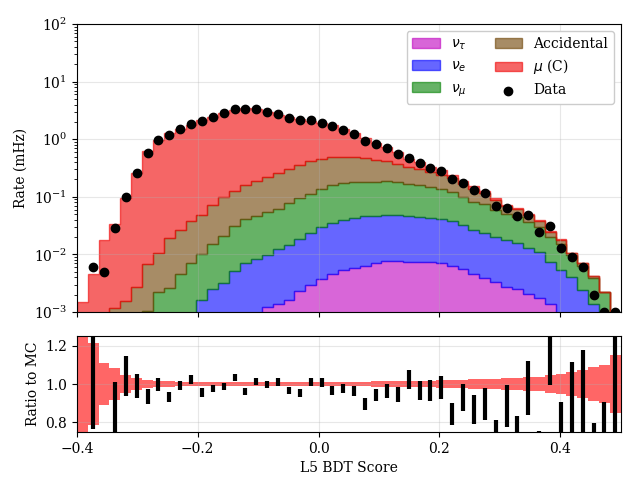
\includegraphics[width=0.9\linewidth]{BDT_Score_log.png}
		\caption[The L5 BDT Score]{The distribution of the BDT decision scores used at L5. A burn sample of 14 days is used to test the data. A cut is again applied at 0.04 to remove a significant fraction of atmospheric muon background events.}
	\label{fig:L5_bdt_log}
\end{figure}

The six variables described in the GRECO Level 5 are again used to train a BDT. 
At the time of training, updated versions of both the GENIE and CORSIKA simulations were provided as part of a ongoing upgrade of the IceCube simulation.
The L5 BDT was trained using simulation files containing the then-newly available Vuvuzela V1 noise model and an updated version of the GENIE Monte Carlo generator.

A set of fifteen variables were tested.
At each step of the training, the least important variable was removed to limit the possible effects of overtraining.
The process continued until changes in the cut efficiency larger than 1\% were observed, resulting in a BDT containing the six most important variables.

The distribution of BDT decision scores is shown in \ref{fig:L5_bdt_log}. 
The data and simulation show good agreement in the muon-dominated region.
In the signal region, the data statistics is low, but the rates are consistent between data and simulation.

The large number of atmospheric muon events at Level 5 preclude the use of more power likelihood reconstructions.
In order to use these additional tools, at least 90\% of the atmospheric muon events must be removed from the sample.
A cut is placed at a score of 0.04, which gives approximately 95\% background rejection with reduction of 30\% to all neutrino rates.
While this is a significant loss in neutrino events, the reduction in rate reduces the computational burden for the processing at the next cut level.

\subsection{Rates at Level 5}
\begin{table}[]
\centering
\begin{tabular}{@{}llllll@{}}
\toprule
Type         & \multicolumn{3}{c}{IceCube Processing} & GRECO  &       \\
             & Any Filter   & DC Filter  & Low-en L3  & L4     & L5    \\ \midrule
CORSIKA      & 990598       & 9178       & 969.82    & 50.511 & 4.100 \\
MuonGun      & 60669        & 2982       & 442.50    & 33.562 & 3.022 \\
Accidentals  & 35855        & 8117       & 283.560    & 11.963 & 1.799 \\
$\nu_e$      & 1.842        & 1.721      & 1.262      & 0.783  & 0.544 \\
$\nu_{\mu}$  & 11.317       & 6.360      & 4.758      & 2.503  & 1.629 \\
$\nu_{\tau}$ & 0.293        & 0.270      & 0.206      & 0.134  & 0.103 \\ \midrule
MC Total*    & 1026466      & 17303      & 1260       & 65.893 & 8.176 \\
Data         & 1154426      & 19092      & 1092       & 68.592 & 7.422 \\ \bottomrule
\end{tabular}
\caption{The event rates after the Level 5 cuts in GRECO.  The total simulated rate is calculated using CORSIKA events and ignoring MuonGun. The data rate is estimated from a burn sample of 14 days. Rates are given in mHz.}
\label{tab:event_rates_L5}
\end{table}

After the GRECO Level 5 cuts, the event rates for the atmospheric muons are a factor of 3x larger than the neutrino flux. 
The rate from accidental triggers in the detector is comparable to the muon neutrino rate.
The tau neutrino rate is more than an order of magnitude smaller than the muon rates, making up less than 2\% of the total rate.
Additonal cuts are needed in order to lower both sets of background below the neutrino rate.
















\graphicspath{{chapters/greco/images/level6/}}
\section{GRECO Level 6 Cuts}
\label{sec:level6}
Unlike previous levels, the GRECO L6 does not rely on a trained boosted decision tree.
The choice was made due to concerns about the significantly limited background simulation.
Such a limitation could lead to overtraining, a situation difficult to test with few simulated events.

Two cuts are applied to the sample at GRECO Level 6 for the removal of the remaining accidental triggers.
An additional three cuts are applied to reduce the muon background rate.

\subsection{Rejection of Accidental Events at L6}

\subsubsection{Fill-Ratio at L6}
\begin{figure}[h]
	\centering
		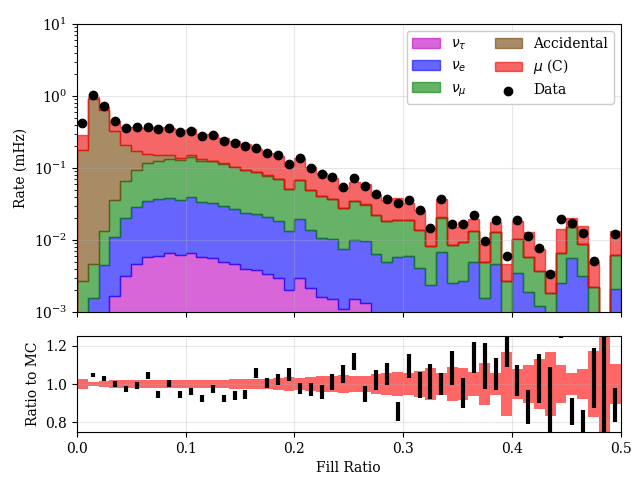
\includegraphics[width=0.9\textwidth]{FillRatio.png}
		\caption[Fill-Ratio]{The fill-ratio distribution. Note the excess of events at low values, a region dominated by the accidental triggers due to detector noise in simulation. A cut is applied at 0.05 to remove these accidental triggers.}
	\label{fig:fill-ratio}
\end{figure}

After GRECO Level 5, the accidental trigger rate is significantly larger than the expected rate of neutrinos.
While the rate of these accidental triggers is low at this stage relative to the rate at L3, they form an important background to the remaining set of neutrino events.
In reduce the number of accidental triggers reaching the tau neutrino appearance analysis, two cuts are introduced to separate signal neutrinos from the accidental background.

The first of these cuts, the \emph{fill-ratio}, is a variable typically used in the search for high energy cascades \cite{IceCube-ICRC2013,IceCube-IC22-Astro} by quantifying the compactness of hits within an event.

Fill-Ratio begins with a reconstructed vertex and pulse series.
In the case of the GRECO Level 6, the first hit position in DeepCore within a STW+SRT cleaned pulse series is used as an event vertex.
Both the pulse series and the event vertex are used in the fill-ratio calcuation.

A radius is computed using the provided information.
Many options are available for the caclulation of different radii, including calculations using the mean or variance of the distance between the pulses and the vertex, a parametrized radius calculation using the number of hit DOMs, and a calculation using a previously reconstructed energy.
Each configuration was tested in GRECO Level 6 with the calculation using the mean distance from the vertex showing the most promise.

\begin{equation}
	r_{Fill-Ratio} = A \left|\left|\frac{\sum_i^{hits} \left(\vec{x_i}-\vec{x}_{vertex}\right)}{N_{hitDOMs}}\right|\right|
\end{equation}

where $A$ is a configurable scale factor. 
The algorithm next indentifies all DOMs contained with a sphere centered on the provided vertex with a radius of $\bar{r}_{Fill-Ratio}$.
The fill-ratio value is then given by the ratio of contained DOMs observing a pulse to the total number of contained DOMs.

\begin{equation}
	f = \left.\frac{N_{hit}}{N_{DOMs}}\ \right\rvert_{\ \left|\left|\vec{r}\right|\right| < r_{FR}}
\end{equation}

This results in a measure of the compactness of a hypothetical cascade, where we expect the resulting hit distribution to be approximately spherically symmetric.
An approximately spherically symmetric cascade-like event will completely fill the fill-ratio sphere, resulting in a value near 1.0.
An extended, track-like event will have hits that are, on average, further from the starting vertex, leading to a large value of $\bar{f}_{Fill-Ratio}$, a large number of contained DOMs, and a small value of the fill-ratio.

In the context of high energy events, the fill-ratio provides good separation between cascade-like and track-like events.
Fill-ratio has not previously been used in low energy analyses, however, due to the short muon tracks of muon neutrino interactions in the 20~GeV region important for atmospheric oscillations.
At GRECO Level 6, fill-ratio has been tested to identify neutrino and atmospheric muon events with no significant separating power observed.

Sgnificant separating power was observed between the neutrino events and accidental triggers, however.
The accidental triggers include pulses throughout the detector with no clustering in the event, unlike events caused by muon or neutrino interactions, which typically have some type of clustering of pulses around the interaction position.
These events receive a large radius due to this lack of clustering and a correspondingly small value of the fill-ratio.
A choice of A=1.6 and the radius calculated using the mean distance between the first hit and all other cleaned pulses gives the separating power shown in Figure~\ref{fig:fill-ratio}.

The observed separation at a value of 0.05 allows up to one order of magnitude of reduction in the rate of accidental triggers with a relatively small reduction in signal rate of approximately 10\%.
The use of fill-ratio reduces the number of accidental triggers expected below the neutrino rate.


\subsubsection{The Number of Hit DOMs}
\begin{figure}[h]
	\centering
		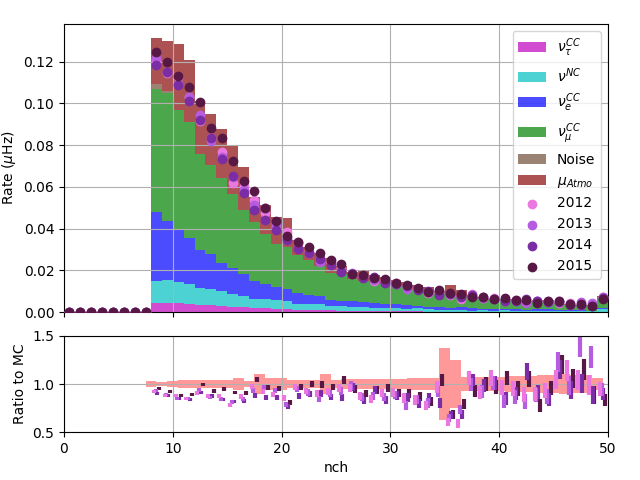
\includegraphics[width=0.9\textwidth]{nch.png}
		\caption[The number of hit DOMs at GRECO Level 6]{The number of hit DOMs in the STW+SRT cleaned pulses series at GRECO Level 6. At least 8 hit DOMs are required for the reconstruction performed at GRECO Level 7. Events with fewer than 8 hits are removed during Level 6, coincidentally reducing the number of accidental triggers expected.}
	\label{fig:nchannel}
\end{figure}

The final reconstruction used in this analysis, Pegleg, is discussed in Section~\ref{subsec:pegleg_reco}.
Like the SPE reconstruction used at Level 5, the Pegleg reconstruction requires a minimum number of hit DOMs in order to converge.
In order to prepare for the reconstruction performed at GRECO Level 7, events with fewer than 8 hit DOMs in the STW+SRT cleaned DeepCore pulse series are removed from the selection.

The distribution of the number of hit DOMs is shown in Figure~\ref{fig:nchannel}.
This removal is performed in order to prepare for the Pegleg reconstruction, but it also removes a significant number of accidental triggers from the selection.
The accidental triggers make up about 0.3\% of events in the sample following the combination of this cut as and the fill-ratio cut.



\subsection{Rejection of Atmospheric Muon Events at L6}
\label{subsubsec:corridorcut}

\subsubsection{CorridorCut}
\begin{figure}[h]
	\centering
		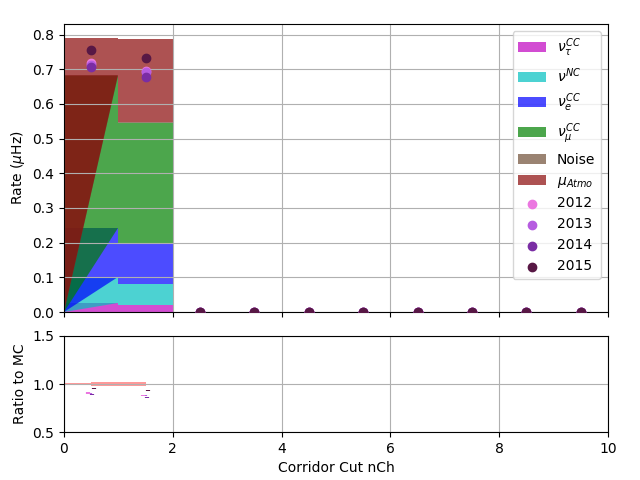
\includegraphics[width=0.9\textwidth]{Corridor_Cut_nCh.png}
		\caption[Number of hit DOMs found by CorridorCut]{The number of hit DOMs discovered along one of the various "corridors" in the detector. Events with at least two hit DOMs discovered along a corridor are removed.}
	\label{fig:corridorcut}
\end{figure}

\begin{figure}
\centering
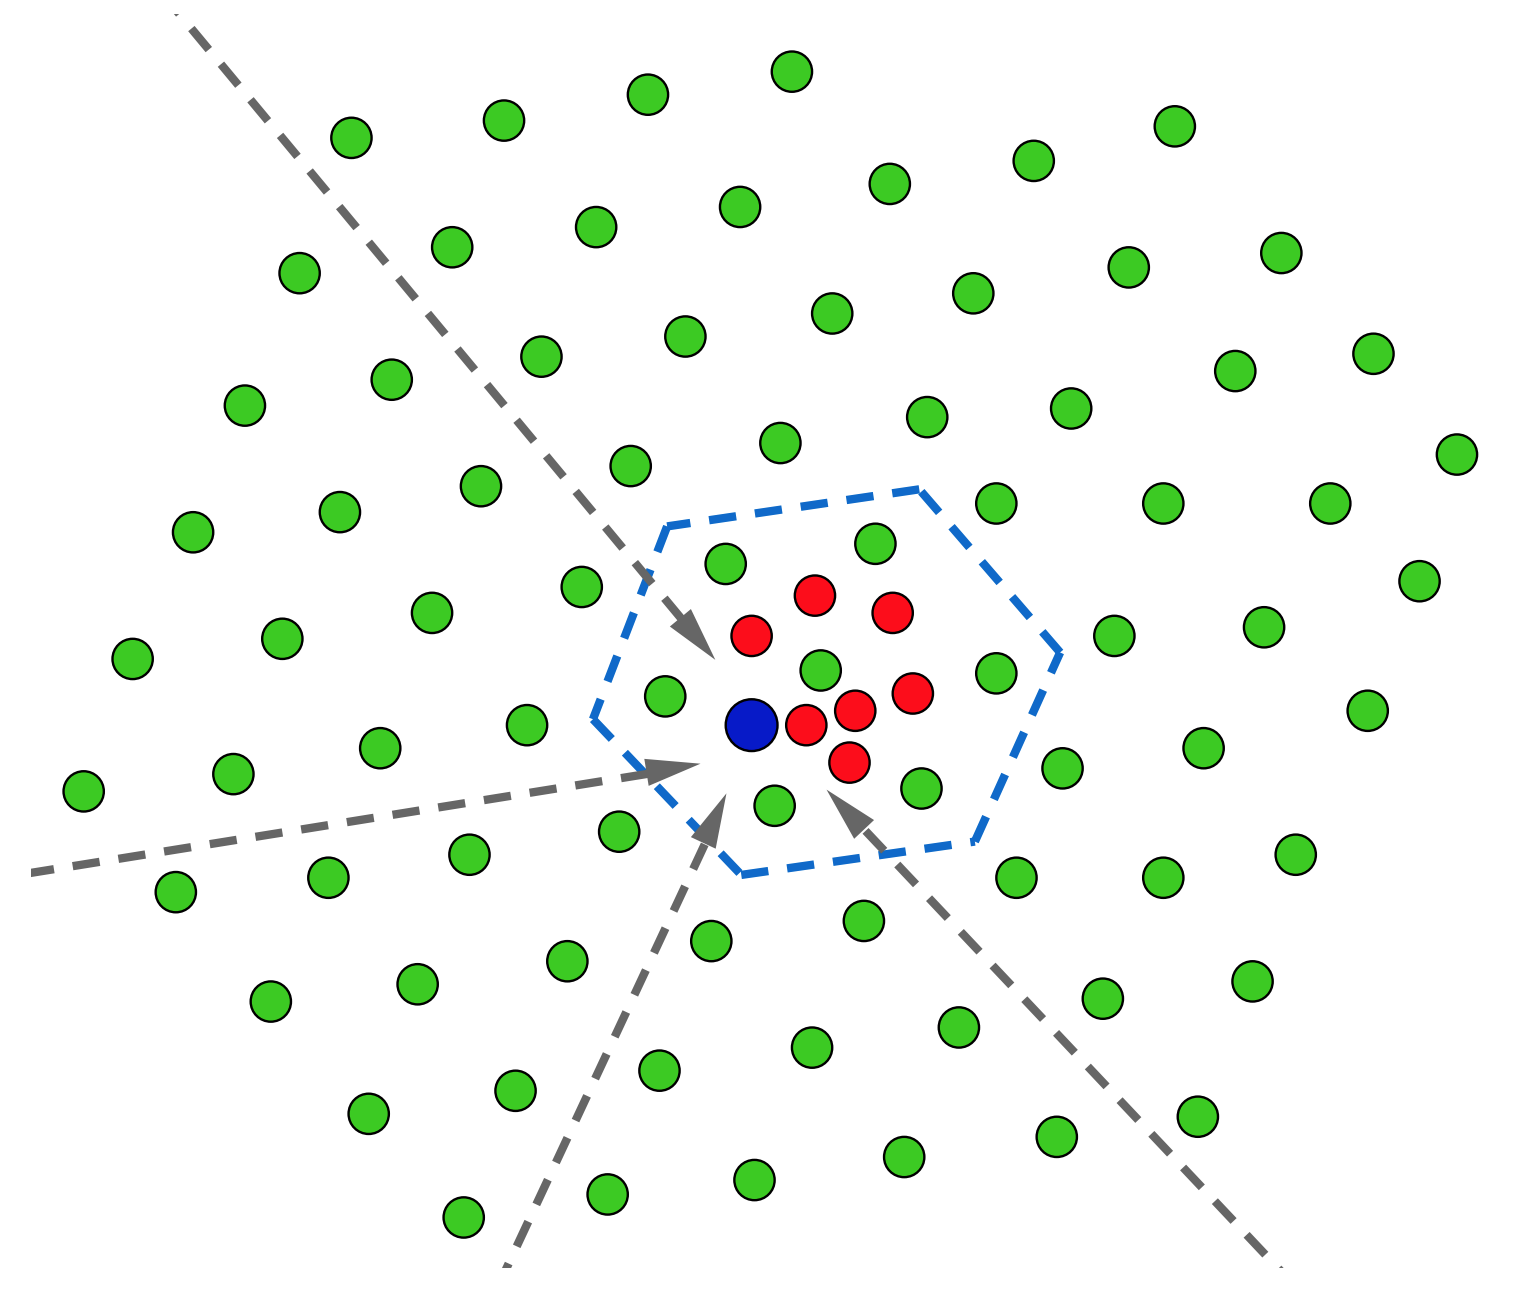
\includegraphics[width=0.7\textwidth]{corridorcut_diagram.png} 
\caption[Example of Corridors into DeepCore]{An example of "corridors" into the DeepCore fiducial volume. Muons may pass into the fiducial volume, outlined in blue, undetected by following the paths indicated by the dashed lines. Image from \cite{Thesis-Dunkman}.}
\label{fig:corridorcut_diagram}
\end{figure}

The remaining atmospheric muon background after the GRECO Level 5 processing show strong selection bias, with few events remaining showing clear tracks in the veto region.
In the past, minimum-ionizing muons were discovered to be leaking into the DeepCore fiducial volume along \emph{corridors}, lines connecting the inner part of the detector to the outer edge without crossing any strings.
These events pass between strings and leave little trace in the form of identifiable hits in the outer detector.
Examples of these corridors are shown in Figure~\ref{fig:corridorcut_diagram}.

In order to identify these muons, a cut was developed to look along pre-defined corridors for SLC hits correlated with pulses in DeepCore.
A CoG of the event is calculated from the STW+SRT cleaned DeepCore pulse series.
The string nearest the CoG is used to choose a set of 'corridor' strings to check for the event.
The number of hit DOMs found on the corridor strings in an uncleaned pulse series is returned.

Due to the effects of random detector noise, a cut limiting the number of discovered corridor hits to 0 would result in a significant loss of signal events.
Instead, one hit is allowed, with two or more discovered DOMs leading to the removal of the event from further processing.
At this stage, there are few events due to atmospheric muons with detectable energy in the veto, resulting in the removal of few events.
The events removed, however, are dominated by atmospheric muons, as seen in FIgure~\ref{fig:corridorcut}.

\subsubsection{FiniteReco Starting Containment}
\begin{figure}[h]
\centering
\begin{tabular}[b]{c}
  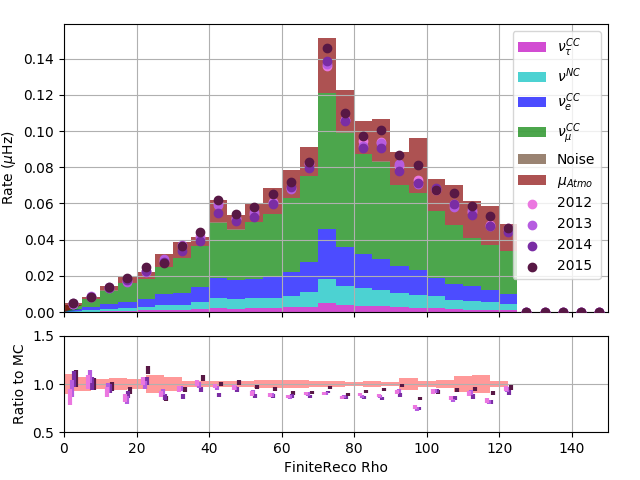
\includegraphics[width=0.45\linewidth]{FiniteReco_Rho.png} \\
  \small (\textbf{\color{ctcolormain}a}) $\rho_{FiniteReco}$
\end{tabular} \hspace{2pt}
\begin{tabular}[b]{c}
  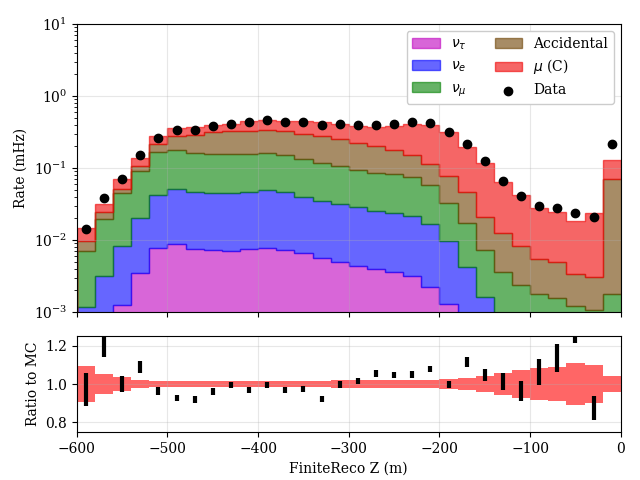
\includegraphics[width=0.45\linewidth]{FiniteReco_Z.png} \\
  \small (\textbf{\color{ctcolormain}b}) $Z_{FiniteReco}$
\end{tabular}
\caption[The FiniteReco Containment Cuts]{The FiniteReco containment cuts. Note the excess of muons at the top and outer edge of the DeepCore fiducial volume.}%
\label{fig:finitereco_cuts}%
\end{figure}

\begin{figure}
\centering
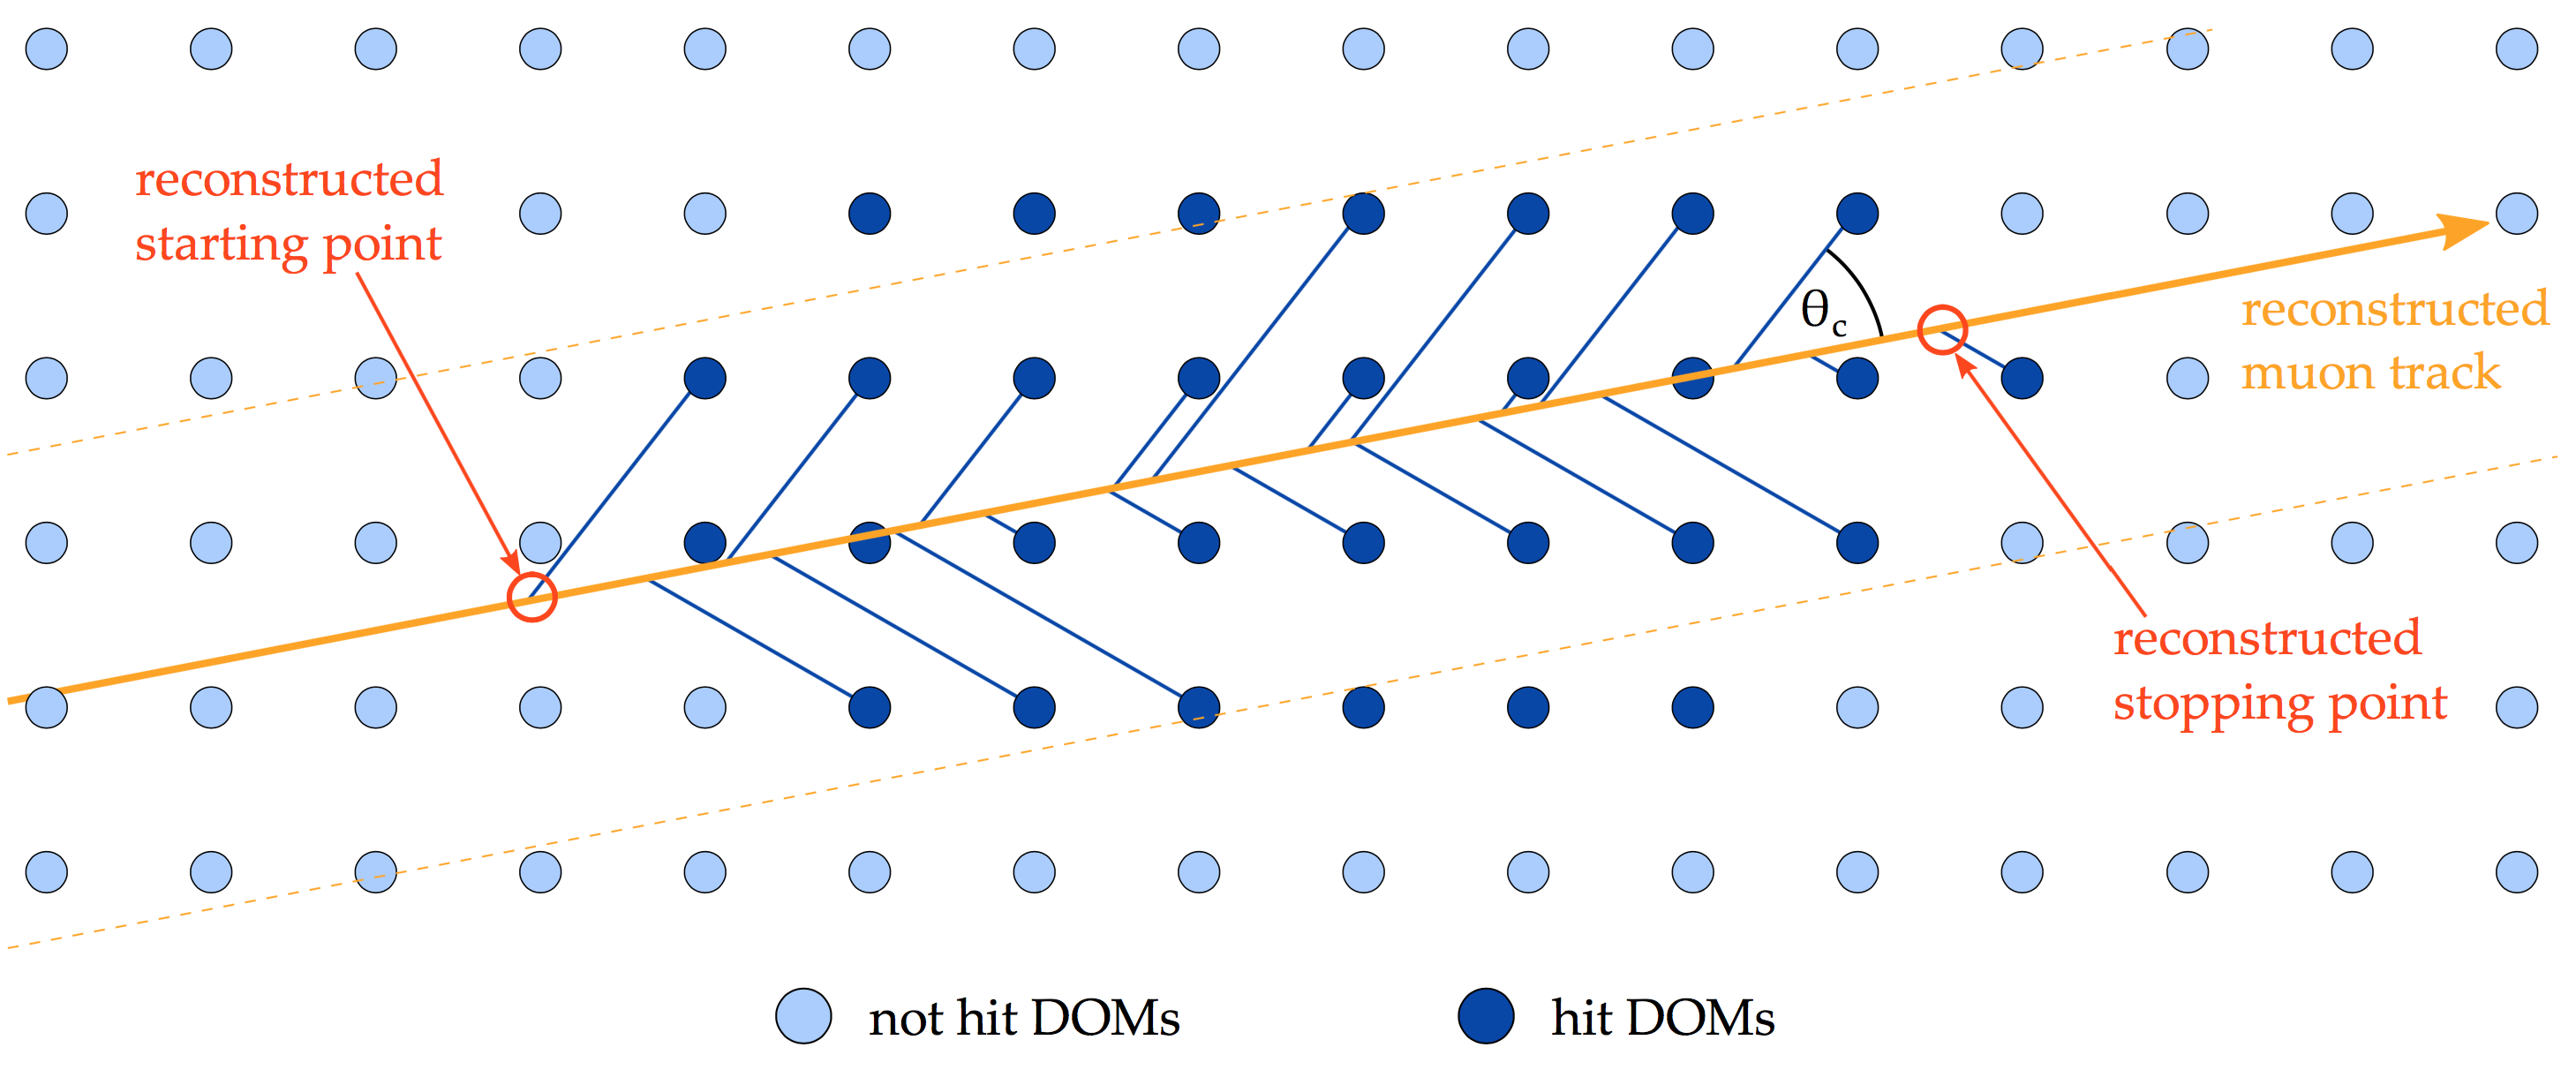
\includegraphics[width=0.9\textwidth]{finitereco_diagram.png} 
\caption[Diagram Describing the FiniteReco Method]{The FiniteReco starting and endpoint reconstruction method. FiniteReco uses an existing muon track reconstruction and the collection of hit DOMs to estimate the starting and end point of the muon track. Diagram from \cite{Thesis-Euler}.}
\label{fig:finitereco_diagram}
\end{figure}

The SPE reconstruction used in L5 was created using an infinite muon hypothesis. 
In order to refine this reconstruction, the \emph{FiniteReco} algorithm is employed.

FiniteReco is a module that accepts a previous reconstruction and a given set of pulses \cite{Thesis-Euler}.
The start and end point of the muon track may be estimated by assuming light is emitted from the track at the Cherenkov angle.
FiniteReco does not change the position or direction of the seed track.
In the GRECO Level 6 processing, the SPE reconstruction from the Level 5 processing is used as a seed in the FiniteReco reconstruction.

The starting position of the resulting reconstructed particle may be used to estimate the interaction point of the particle.
Figure~\ref{fig:finitereco_zVsRho} shows the position of the reconstructed vertex in terms of depth and distance from string 36.
If an event begins outside of the DeepCore fiducial volume, the event is likely to contain a muon and can be removed from the sample.
Cuts are applied at the positions shown, resulting in a significant reduction in the number of muon events expected at Final Level.

\begin{figure}
\centering
\begin{tabular}{cc}
    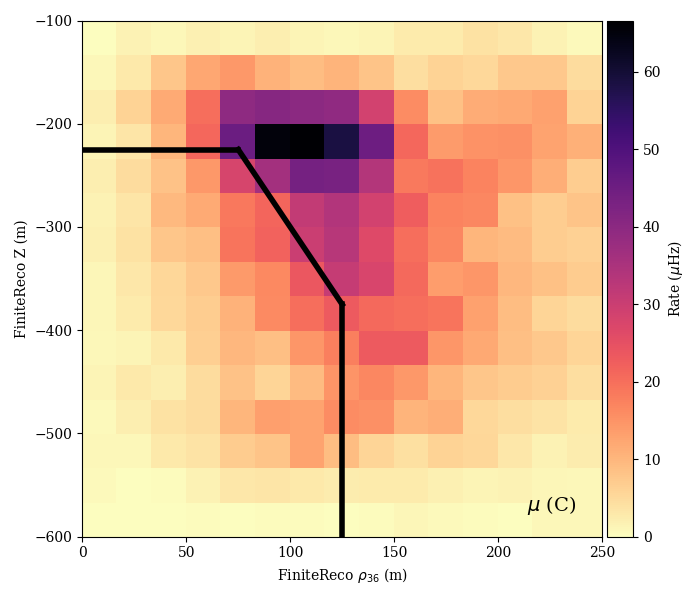
\includegraphics[width=0.45\linewidth]{z_rho_corsika.png} &  
    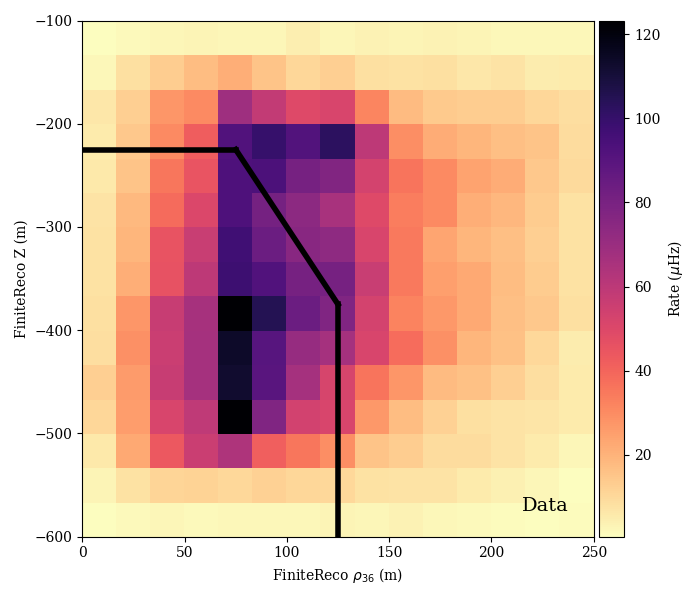
\includegraphics[width=0.45\linewidth]{z_rho_data.png} \\  

    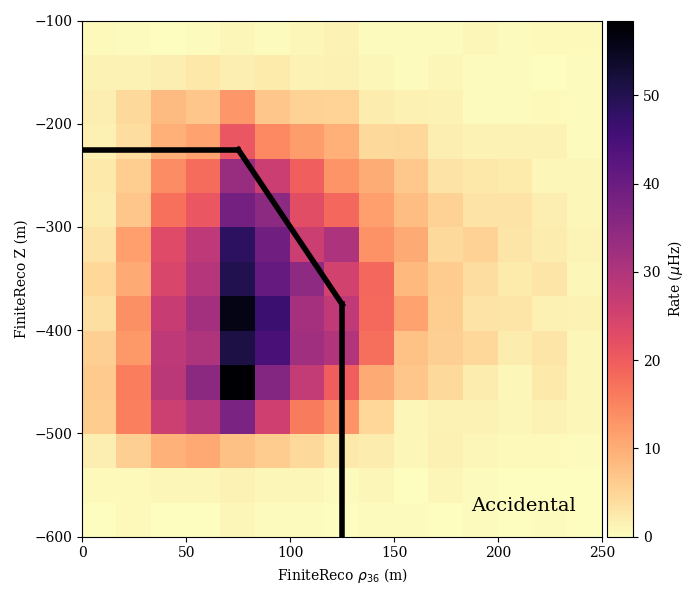
\includegraphics[width=0.45\linewidth]{z_rho_noise.png} &  
    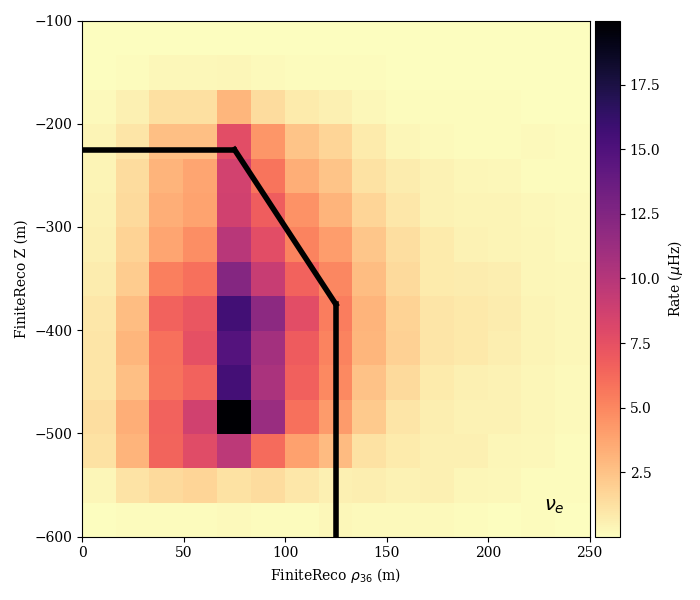
\includegraphics[width=0.45\linewidth]{z_rho_genie_nue.png} \\  

    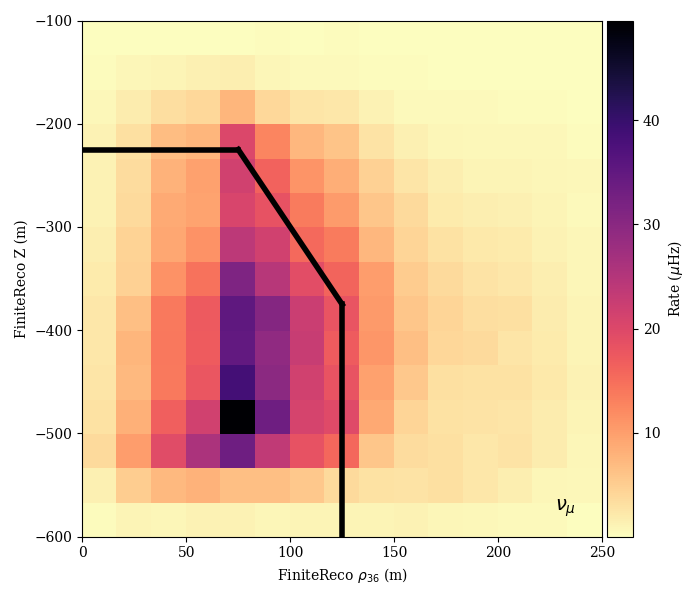
\includegraphics[width=0.45\linewidth]{z_rho_genie_numu.png} &  
    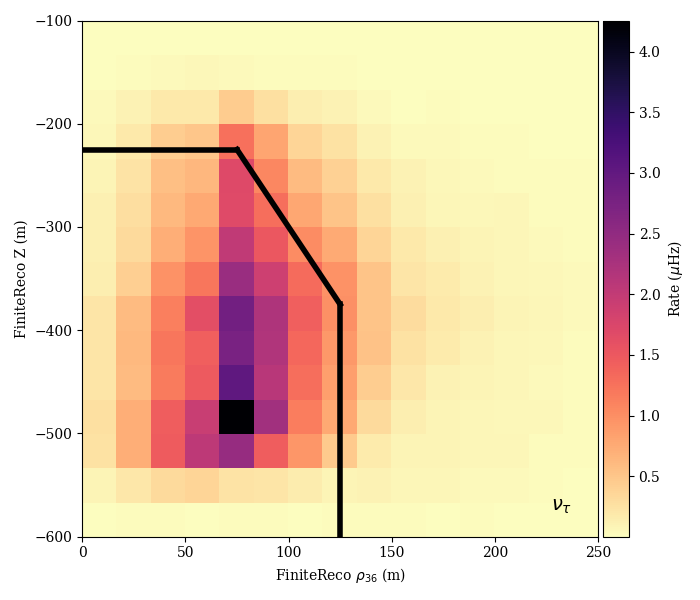
\includegraphics[width=0.45\linewidth]{z_rho_genie_nutau.png} \\ 
\end{tabular}
\caption[The FiniteReco containment cut applied at GRECO Level 6]{The FiniteReco containment cut for each of the channels. The cut itself is shown with the black line. The atmospheric muons, modeled with the CORSIKA generator, are reconstructed at the top of the DeepCore volume.}
\label{fig:finitereco_zVsRho}
\end{table}
\end{figure}


\subsection{Rates at Level 6}
\begin{table}[]
\centering
\begin{tabular}{@{}lllllll@{}}
\toprule
Type         & \multicolumn{3}{c}{IceCube Processing} & \multicolumn{3}{c}{GRECO} \\
             & Any Filter   & DC Filter  & Low-en L3  & L4      & L5     & L6     \\ \midrule
CORSIKA      & 990598       & 9178       & 969.818    & 50.511  & 4.100  & 0.443  \\
MuonGun      & 60669        & 2982       & 442.493    & 33.562  & 3.022  & 0.315  \\
Accidentals  & 35855        & 8117       & 283.559    & 11.963  & 1.799  & 0.102  \\
$\nu_e$      & 1.842        & 1.721      & 1.262      & 0.783   & 0.544  & 0.362  \\
$\nu_{\mu}$  & 11.317       & 6.360      & 4.758      & 2.503   & 1.629  & 1.011  \\
$\nu_{\tau}$ & 0.293        & 0.270      & 0.206      & 0.134   & 0.103  & 0.074  \\ \midrule
MC Total*    & 1026466      & 17303      & 1260       & 65.893  & 8.176  & 1.991  \\
Data         & 1154426      & 19092      & 1092       & 68.592  & 7.422  & 1.841  \\ \bottomrule
\end{tabular}
\caption{The event rates after the Level 6 cuts in GRECO.  The total simulated rate is calculated using CORSIKA events and ignoring MuonGun. Rates are given in mHz.}
\label{tab:event_rates_L5}
\end{table}

After the GRECO Level 6 cuts, the sample is dominated by neutrino events.
The expected muon rate from CORSIKA simulation makes up 22\% of the total sample.
The rate from accidental events is also small, with only 5\% of events due to random detector noise.











\graphicspath{{chapters/greco/images/level7/}}
\section{GRECO Level 7: Final Level}
\label{sec:level7}
The Final Level of the GRECO event selection, \emph{GRECO Level 7}, is the most computationally expensive stage of the selection.
While previous stages have focused on speed, using cuts based on analytic variables or on fast reconstructions using approximations to the scattering of the ice, the GRECO Level 7 employs the Pegleg reconstruction.
This reconstruction is expensive, requiring an average of 10 minutes per event.

The Pegleg reconstruction can be used to define new cuts to further reduce the atmospheric muon rates based on the position of events in the detector.


\subsection{Reconstruction using Pegleg}
\label{subsec:pegleg_reco}
The \emph{Pegleg} reconstruction \cite{Thesis-Martin}, a refinement of previous work \cite{Thesis-Dunkman}, is a low-energy reconstruction that uses a hybrid cascade+muon hypothesis.
The reconstruction returns a total of eight parameters: the position ($x$, $y$, $z$), time ($t$), direction ($\theta$, $\phi$), total energy ($E_{cascade}$) and track length ($L$). 
The total energy of the event is calculated by assuming the muon track is minimally ionizing with an energy loss of 220 MeV/m in ice \cite{Thesis-Dunkman}.

\begin{equation}
\label{eqn:pegleg_energy}
	E_{total} = E_{cascade} + \left(220 MeV/m\right) L
\end{equation} 

The algorithm requires seeds for each of the particle parameters and a collection of hits over which to run.
Pegleg also requires a set of splines describing the expected charge as a function of distance from the emission point.
These splines are created using the CLSim module (see Section~\ref{subsec:clsim}) to directly account for the the scattering and absorption properties of the bulk ice model.

For each particle hypothesis, the event is broken into time steps based on the observed pulses in the event.
At each time step, the expected charge at each DOM is calculated based on the energy and position of the particle hypothesis.
The charge expectation is evaluated for all DOMs, regardless of whether a hit is observed or not.
The total likelihood of the hypothesis is then the product of the likelihoods at each DOM.

The likelihood space itself typically possesses multiple local minima due to the small number of hits.
The fit is performed using the MultiNest minimizer package \cite{MultiNest} in order to handle the complex likelihood space.
The likelihood at each point is used to estimate the underlying likelihood space and produces new hypotheses for testing using importance nested sampling \cite{MultiNest-ImportanceSampling}.

Given the large dimensionality of the 8D parameter space, significant computational power is required for the fit.
Simplifications are introduced to reduce the computational requirements of the Pegleg reconstruction.
Track lengths are limited to integer multiples of the track length used to produce the ice model spline functions.
While this requirement is lifted in newer versions of the software \cite{Thesis-Martin}, that change has not yet propagated to the current GRECO events.
In addition, only DOMs within 150~m of the current particle position are evaluated to find the expected charge.
All other DOMs are assumed to have an expected charge consistent with noise rates.
This assumption allows the minimizer to avoid costly calculations of expected charge for distant DOMs at the expense of higher energy event resolutions.

In early versions of the Pegleg fit, the charge of individual pulses is used directly in the likelihood calculations \cite{IceCube-Millipede}.
Following the discoveries discussed in \ref{subsec:pmt_disagreement}, however, the use of the charge was removed \cite{Thesis-Martin}}.
In the version of Pegleg used in the final version of this analysis, a deadtime window of 45~ns is introduced for each DOM directly following a pulse. 
During this window, the DOM may not contribute any further information to the fit.
This changes the reconstruction likelihood from being on the observed charge to being sensitive only to the observation or absence of charge.
Using this modification, disagreements between the data and simulated pulses resulting from mismodeling are be minimized.


\subsection{Containment with Pegleg}
\label{subsec:pegleg_containment}
With a more refined reconstruction, additional constraints on the containment of the starting vertices are possible.
Similar to the work done with FiniteReco at Level 6, the reconstructed $Z$ and $\rho_{36}$ receive three cuts as shown in \ref{fig:pegleg_zVsRho}.

\begin{•}

Once again, events at the top of and near the edge of DeepCore are more likely to be muons.
An additional cut is applied at the bottom of the detector in order to limit the effect of observed discrepancies between data and simulation.
Removing these events results in a 75\% reduction of the atmospheric muon background at a cost of approximately 10\% of the overall neutrino rate.

\begin{figure}
\centering
\begin{tabular}{cc}
    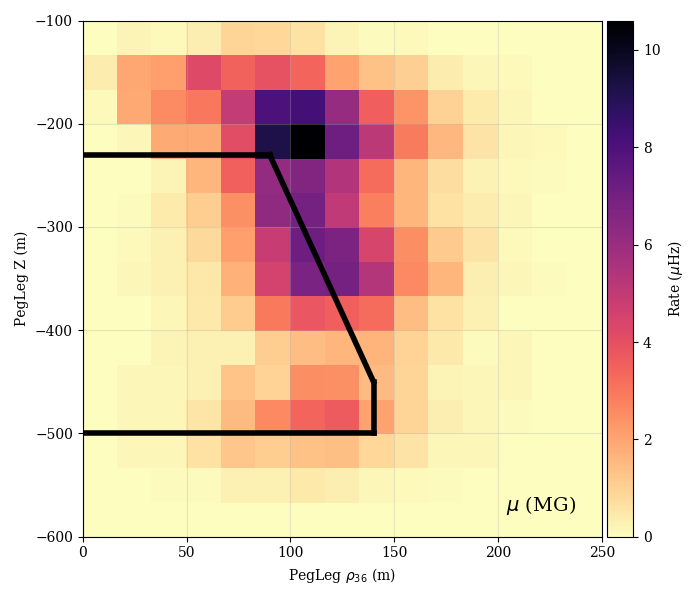
\includegraphics[width=0.45\linewidth]{pegleg_z_rho_muongun.png} &  
    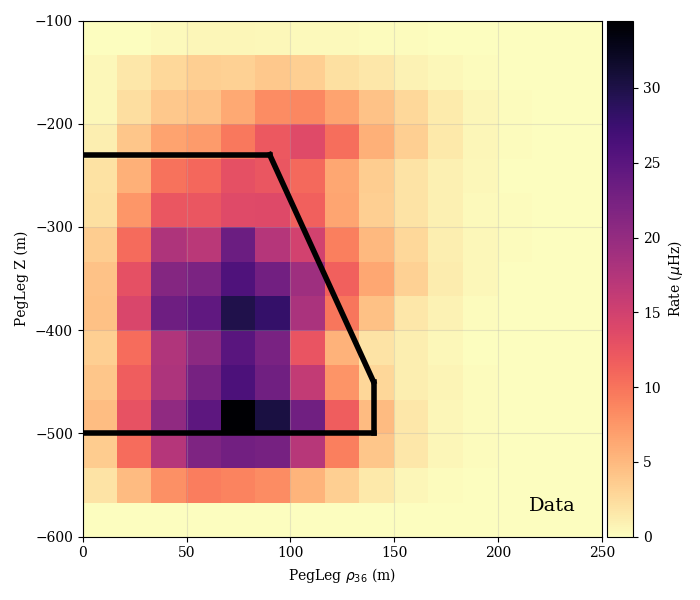
\includegraphics[width=0.45\linewidth]{pegleg_z_rho_data.png} \\  

    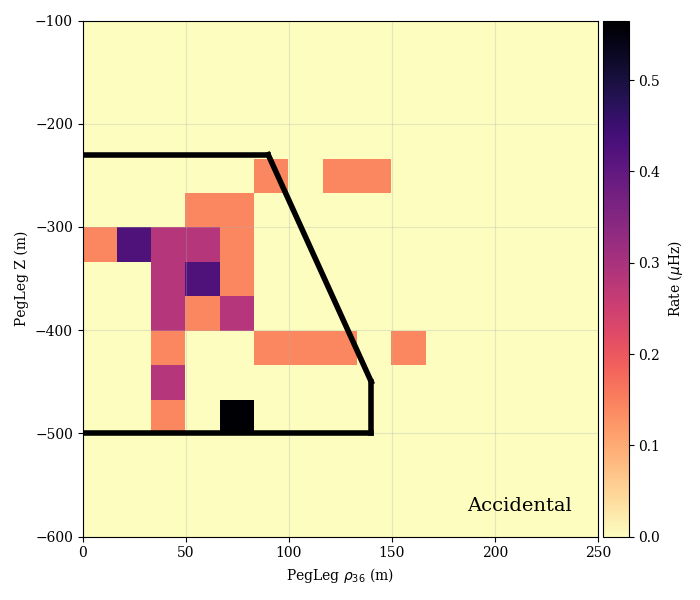
\includegraphics[width=0.45\linewidth]{pegleg_z_rho_noise.png} &  
    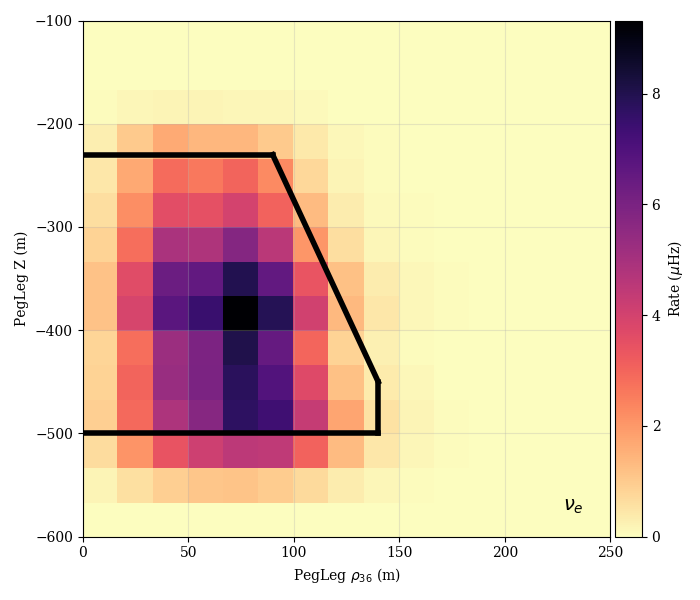
\includegraphics[width=0.45\linewidth]{pegleg_z_rho_genie_nue.png} \\  

    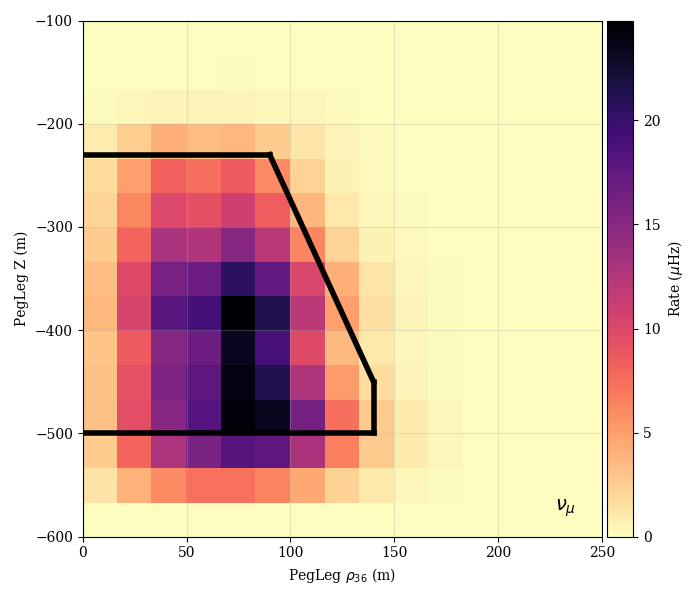
\includegraphics[width=0.45\linewidth]{pegleg_z_rho_genie_numu.png} &  
    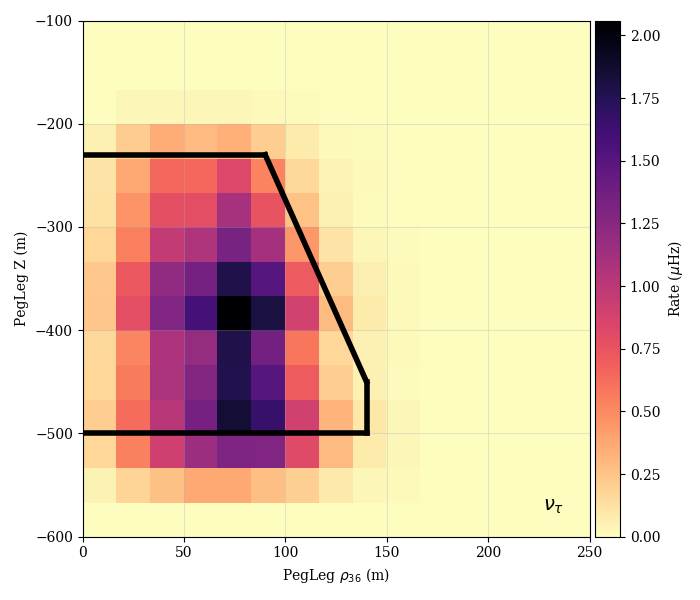
\includegraphics[width=0.45\linewidth]{pegleg_z_rho_genie_nutau.png} \\ 
\end{tabular}
\caption[The Pegleg containment cuts applied at Level 7]{The Pegleg L7 containment cut for each of the channels. The cut is shown with the black line. Note that the atmospheric muons are here represented by the higher-statistics MuonGun sample.}
\label{fig:pegleg_zVsRho}
\end{figure}


\subsection{Other Cuts at L7}
\label{subsec:other_l7_cuts}
Cuts are also applied to the average reconstructed energy per hit DOM and the scatter in the timing distribution of hits, shown together in Figure~\ref{fig:trms_ench}.
The former is expected to yields high values for events dominated by flaring DOMs (Section~\ref{sec:greco_discoveries}) or events where a particle interaction occurs very close to the face of a DOM.
A cut removing events with more than 3 GeV/DOM is applied only to events with fewer than 14 hits, limiting the impact on the neutrino signal events.

The scatter in the hit times is used to identify accidental events, which are not expected to produce hits correlated across DOMs.
The cut, which removes events where the standard deviation of the hit times is larger than 800~ns, is also only applied for events with fewer than 14 hits.
This limits the loss of neutrino events while removing a fraction of the remaining accidental triggers.



\begin{figure}
\centering
\begin{tabular}{cc}
    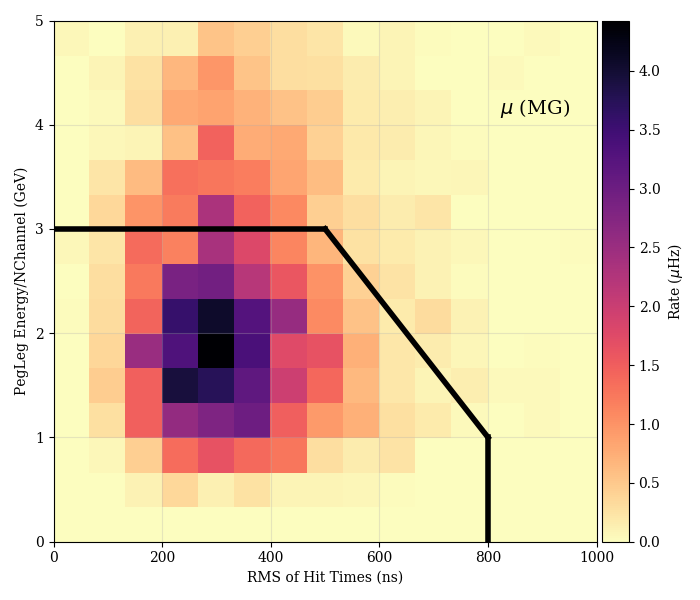
\includegraphics[width=0.45\linewidth]{pegleg_trms_ench_muongun.png} &  
    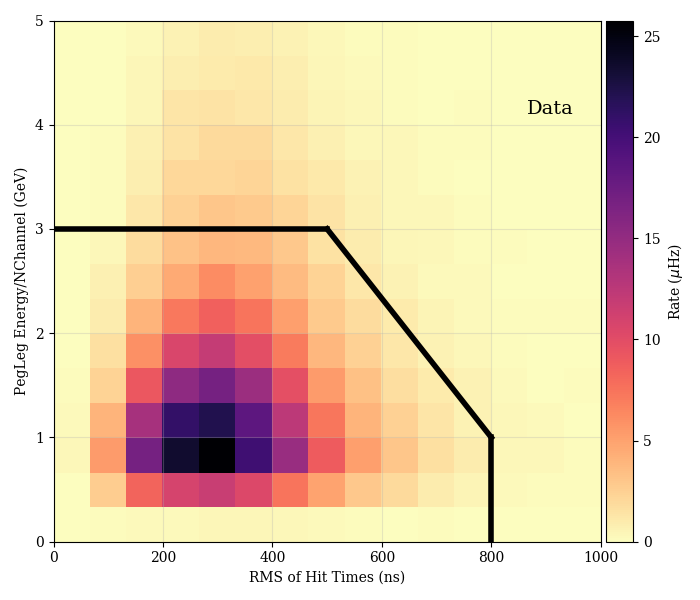
\includegraphics[width=0.45\linewidth]{pegleg_trms_ench_data.png} \\  

    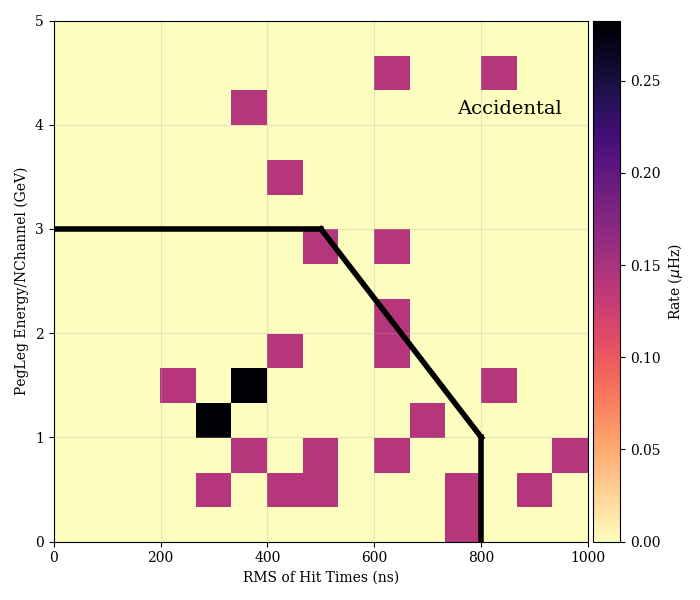
\includegraphics[width=0.45\linewidth]{pegleg_trms_ench_noise.png} &  
    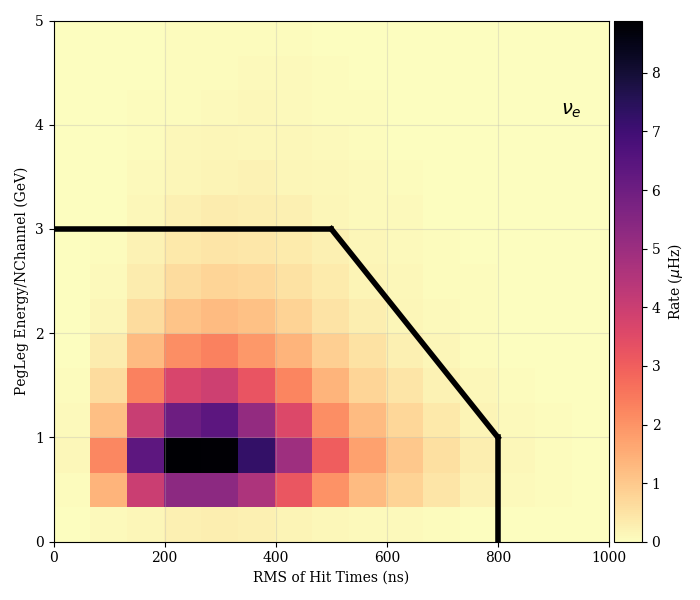
\includegraphics[width=0.45\linewidth]{pegleg_trms_ench_genie_nue.png} \\  

    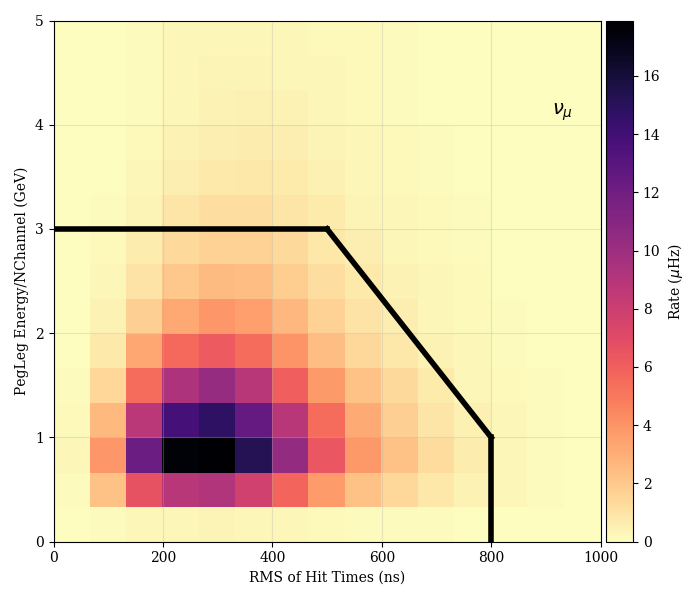
\includegraphics[width=0.45\linewidth]{pegleg_trms_ench_genie_numu.png} &  
    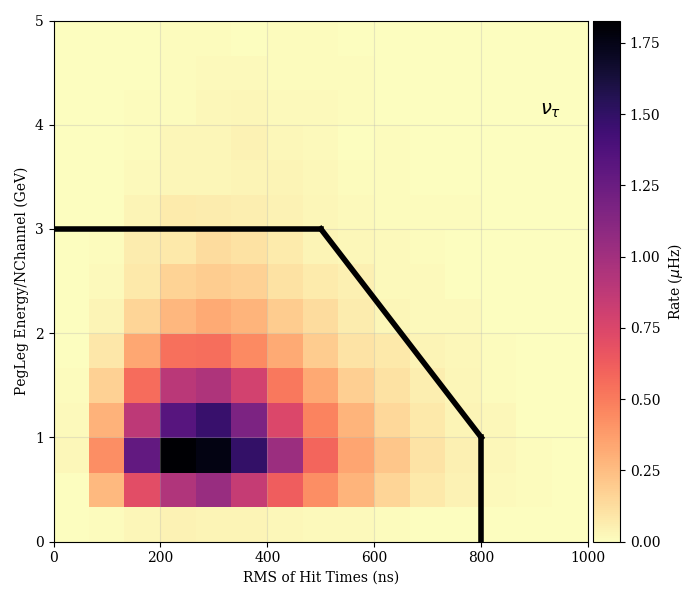
\includegraphics[width=0.45\linewidth]{pegleg_trms_ench_genie_nutau.png} \\ 
\end{tabular}
\caption[The 2D cuts applied to the time and energy variables at Level 7]{The cuts applied to the reconstructed energy per hit DOM and the standard deviation in the hit times. The cuts are designed to remove atmospheric muons and highly scattered events from the selection. The 2D cut shown here is applied only to events with fewer than 14 hit DOMs. }
\label{fig:trms_ench}
\end{figure}


















\graphicspath{{chapters/greco/images/}}
\section{Calibration Discoveries with GRECO}
\label{sec:greco_discoveries}
Checks with the GRECO selection during the search for appearance uncovered disagreements between data and simulation.
Five discoveries made with the selection are discussed here.

\subsection{The Simulation SPE Templates}
\label{subsec:spe_template}
During the development of the GRECO selection, new calibration measurements showed that the SPE peak in data was misaligned.
This SPE peak, a part of the SPE template described for simulation in Section~\ref{subsec:pmtsim}, is used to convert between the pulses of the waveform, in units of millivolts, and the charge units in IceCube, in units of photoelectrons (\emph{PEs}).
The peak is intended to correspond to a value of 1 PE, indicating a single photon interacting at the photocathode of the PMT.
While previous measurements had measured an average SPE template for the detector data, the new calibrations were used to measure the templates for individual DOMs.

The updated calibration measurements showed that the SPE peak used in data was not at 1 PE, but was, on average, at 1.045 PE. 
The IceCube collaboration subsequently corrected the SPE templates for data beginning in the IC86-5 (2015-2016) season, shifting the location of the extracted SPE peak in data from 1.045 PE to 1 PE.
The correction is believed to result in a more accurate extaction of the charge in data.
The simulation SPE template, shown in Figure~\ref{fig:ta0003}, peaked at 1 PE by definition and was not changed.
This shift mirrors effects observed during the fitting of the Vuvuzela V2 model in which a charge scaling variable was introduced to improve agreement with data and simulation (see Section~\ref{sec:vuvuzela_fitting}).

After the correction, analyses searching for high energy neutrinos in the IceCube detector showed improved agreement between data and simulation.
Previous analyses searching for oscillations in DeepCore had observed good agreement between data and Monte Carlo simulations prior to the correction to the SPE template in data \cite{IceCube-Oscillation2013,IceCube-Oscillation2015,IceCube-Oscillation2018}.
In order to evaluate the effect of the correction, the IC86-5 data was processed using the standard GRECO processing scripts.

\begin{figure}
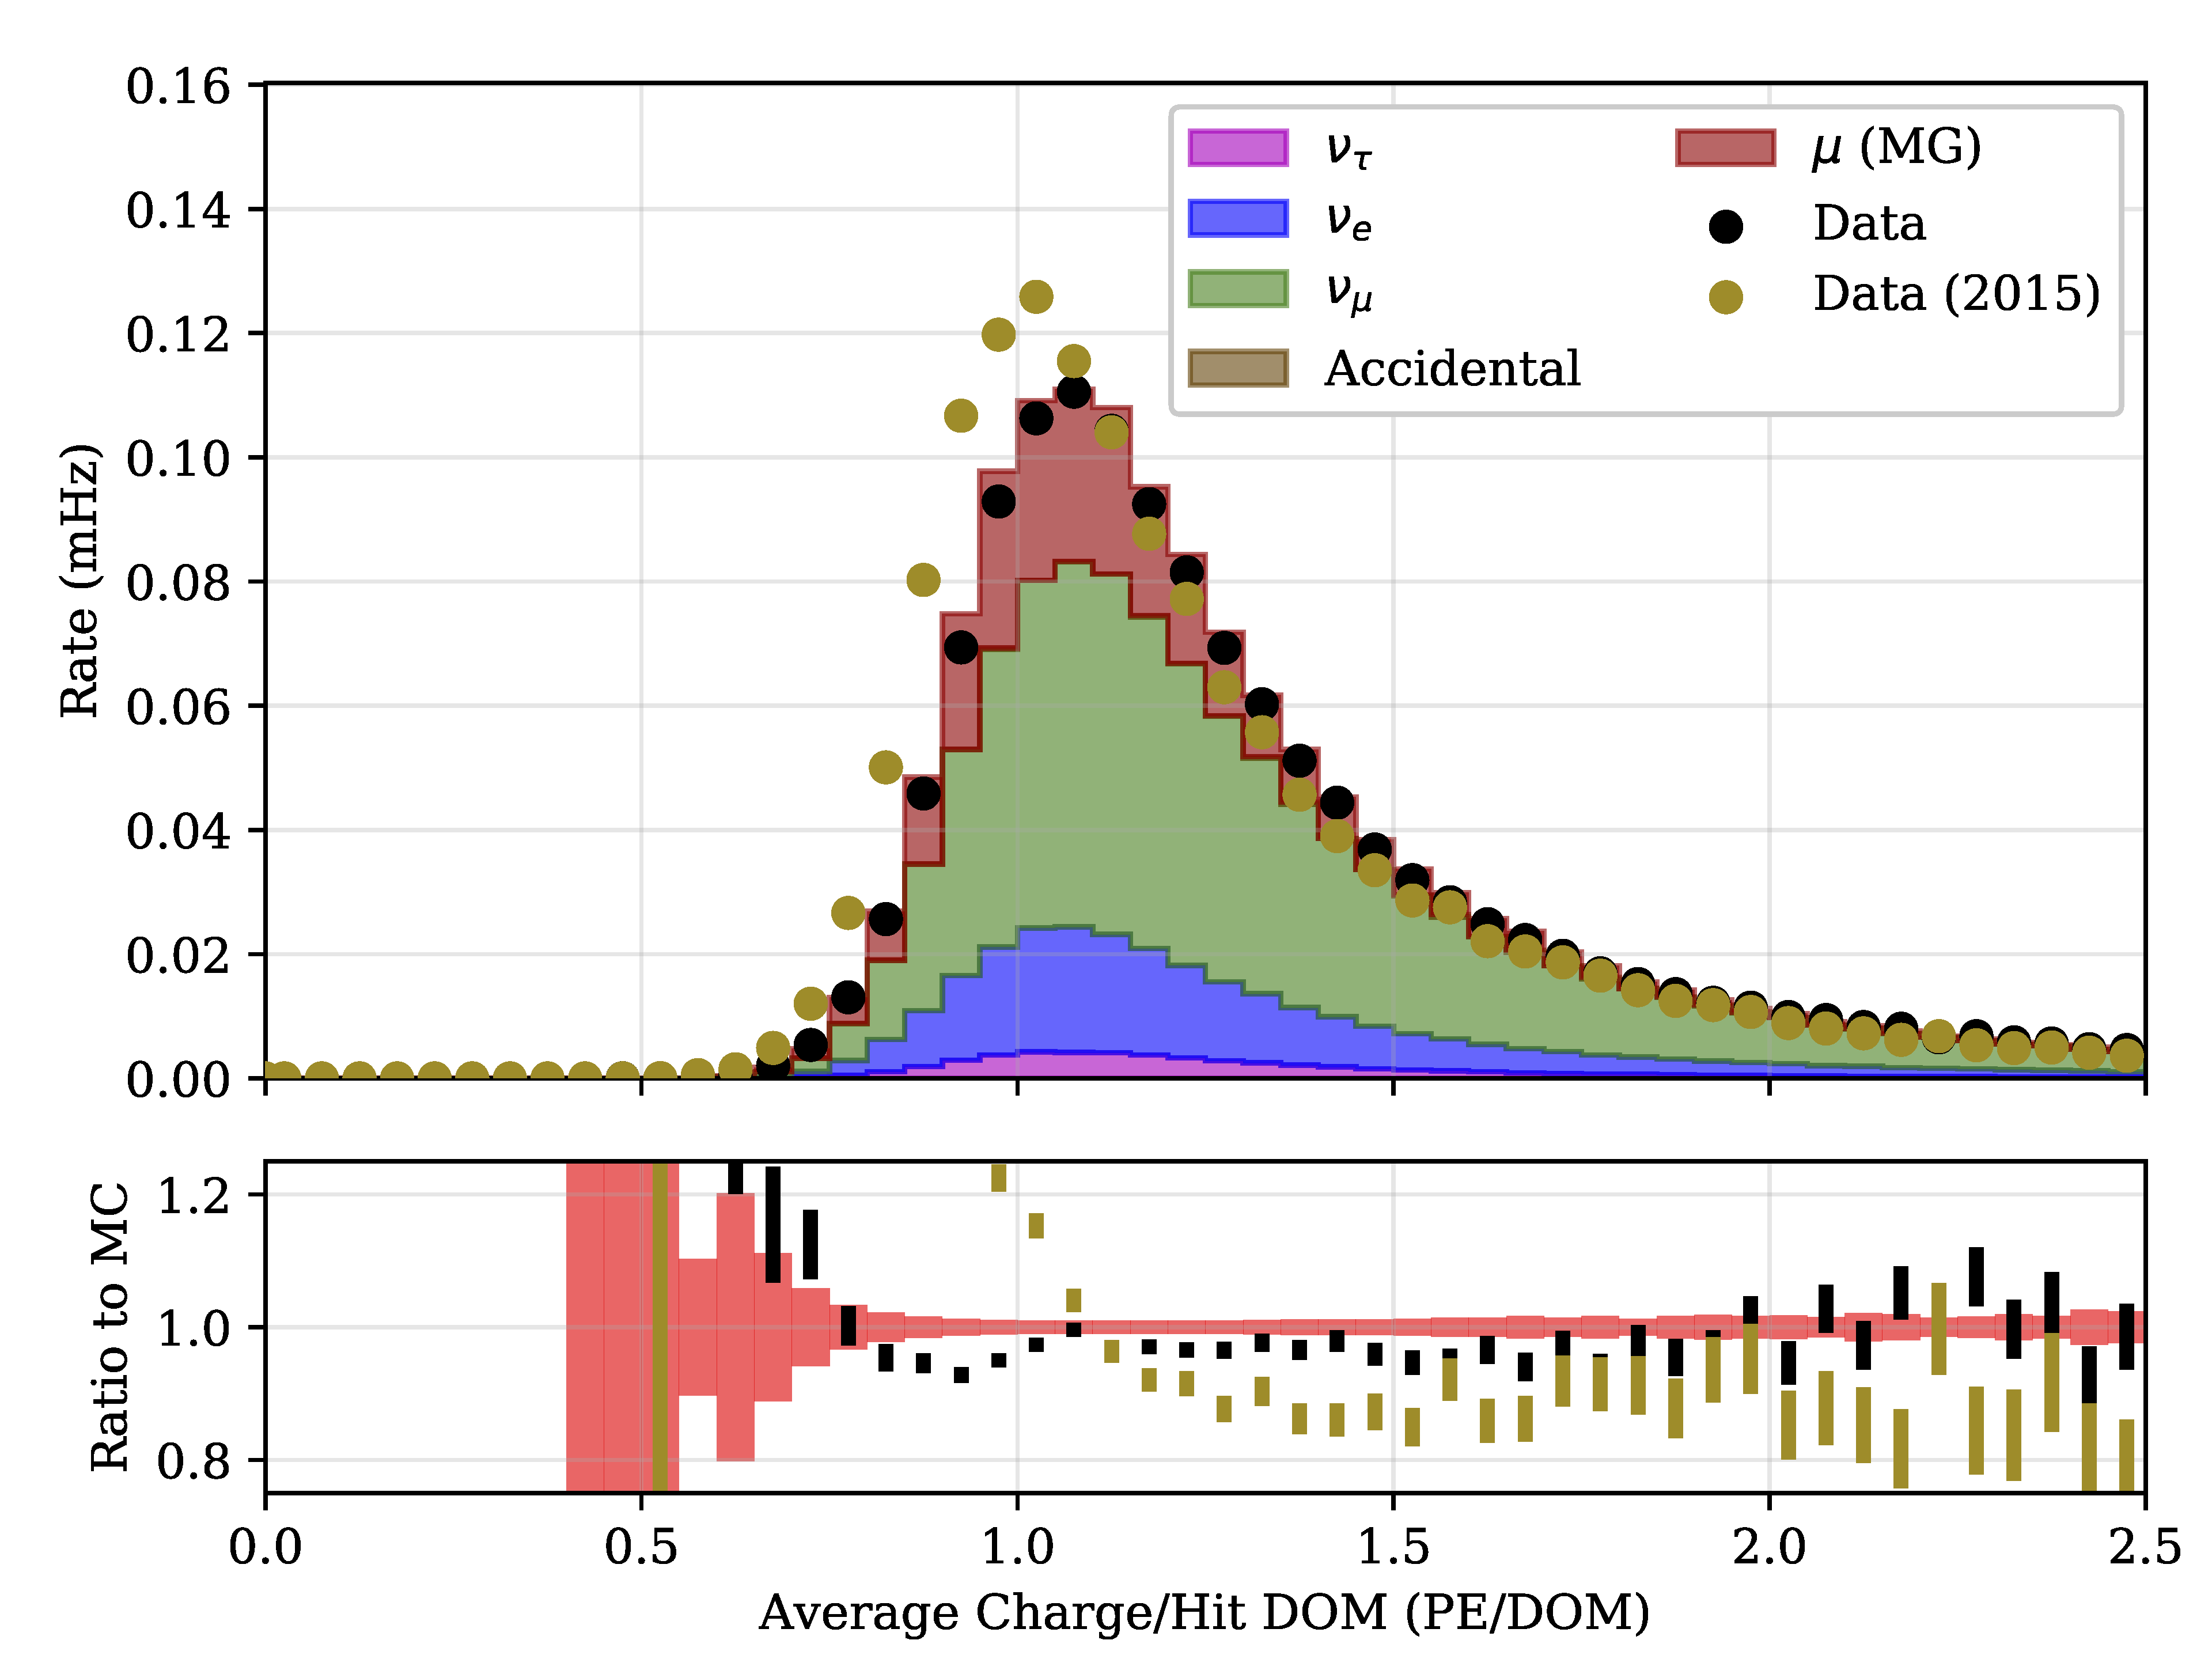
\includegraphics[width=0.9\textwidth]{L7_charge_per_channel.png} 
\caption[The effect of the data SPE correction applied in 2015]{The effects of the SPE correction applied to data in 2015. As expected, the peak of the distribution is closer to 1 PE in the corrected 2015 data (gold circles) than in previous years (black circles). While the simulation showed good agreement with the data taken prior to the recalibration of the SPE peak, the recalibrated data shows marked disagreement. Investigations into this anomaly showed that the SPE templated used in simulation does not accurately model our data.}
\label{fig:q_over_nch}
\end{figure}

At low energies, most observed hits are due to single photons reaching the PMT.
The average charge per DOM is therefore expected to approximately follow the SPE template.
This variable was used to evaluate the effects of the correction at Level 7 of the GRECO selection.

The result is shown in Figure~\ref{fig:q_over_nch}.
As expected, the 2015 data shows a shift downward, with a peak closer to 1 PE.
Unexpectedly, however, the corrected dataset shows substantial disagreement with simulated events.

\begin{figure}
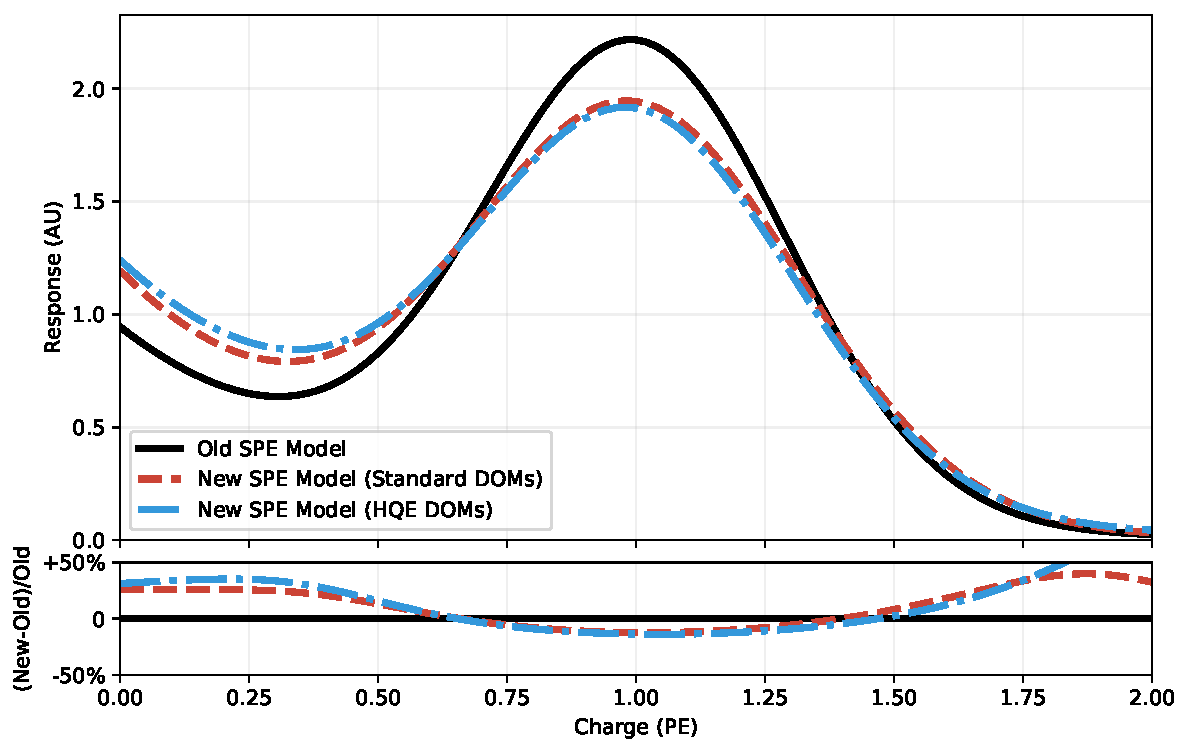
\includegraphics[width=0.9\textwidth]{updated_spe.pdf} 
\caption[A comparison if the old and new SPE templates for simulation]{A comparison of the old SPE template previously used in the simulation of events to the new average templates for the high quantum efficiency DOMs and the standard IceCube DOMs. The new models predict a higher number of pulses with low charge, consistent with the excess observed from the corrected 2015 data in Figure~\ref{fig:q_over_nch}.}
\label{fig:new_spe_templates}
\end{figure}

Investigations of the disagreement showed that the data and simulation disagreed at all cut levels, including low cut levels unrelated to the GRECO selection.
The issue has been identified to be the SPE templates used in the simulation.
The template used is calculated as the average of 118 DOMs measured in the lab prior to deployment \cite{TA0003}.

New work has been performed to apply the SPE templates measured in the data calibrations to the Monte Carlo simulation for all DOMs in the detector.
The new templates, shown in Figure~\ref{fig:new_spe_templates}, predict more hits with low charges, as observed in the 2015 data of Figure~\ref{fig:q_over_nch}.

Due to time contraints, the updated simulation has not been evaluated in the GRECO sample.
In order to reduce the potential disagreement arising between data and simulation due to mismodeled low charges, both the data and simulation have been processed with a version of the Pegleg reconstruction designed to limit the dependence on charge information.


\subsection{Disagreement in PMT Simulation}
\label{subsec:pmt_disagreement}
While investigating charge variables related to the SPE template, additional disagreements were discovered in the PMT simulation.
The first suspected cause  of charge disagreements was erroneous splitting of the waveform during charge extraction.

The SPE template is used to convert the digitized waveforms from the FADC and ATWD into reconstructed photoelectrons consisting of charge and timing information.
While the simulated response is known exactly when extracting pulses, the associated charge response of the DOM in data requires calibration.
Using a mismodeled charge response to extract pulses in the data can result in single photoelectrons being erroneously split into multiple smaller reconstructed pulses.

\begin{figure}
\centering
	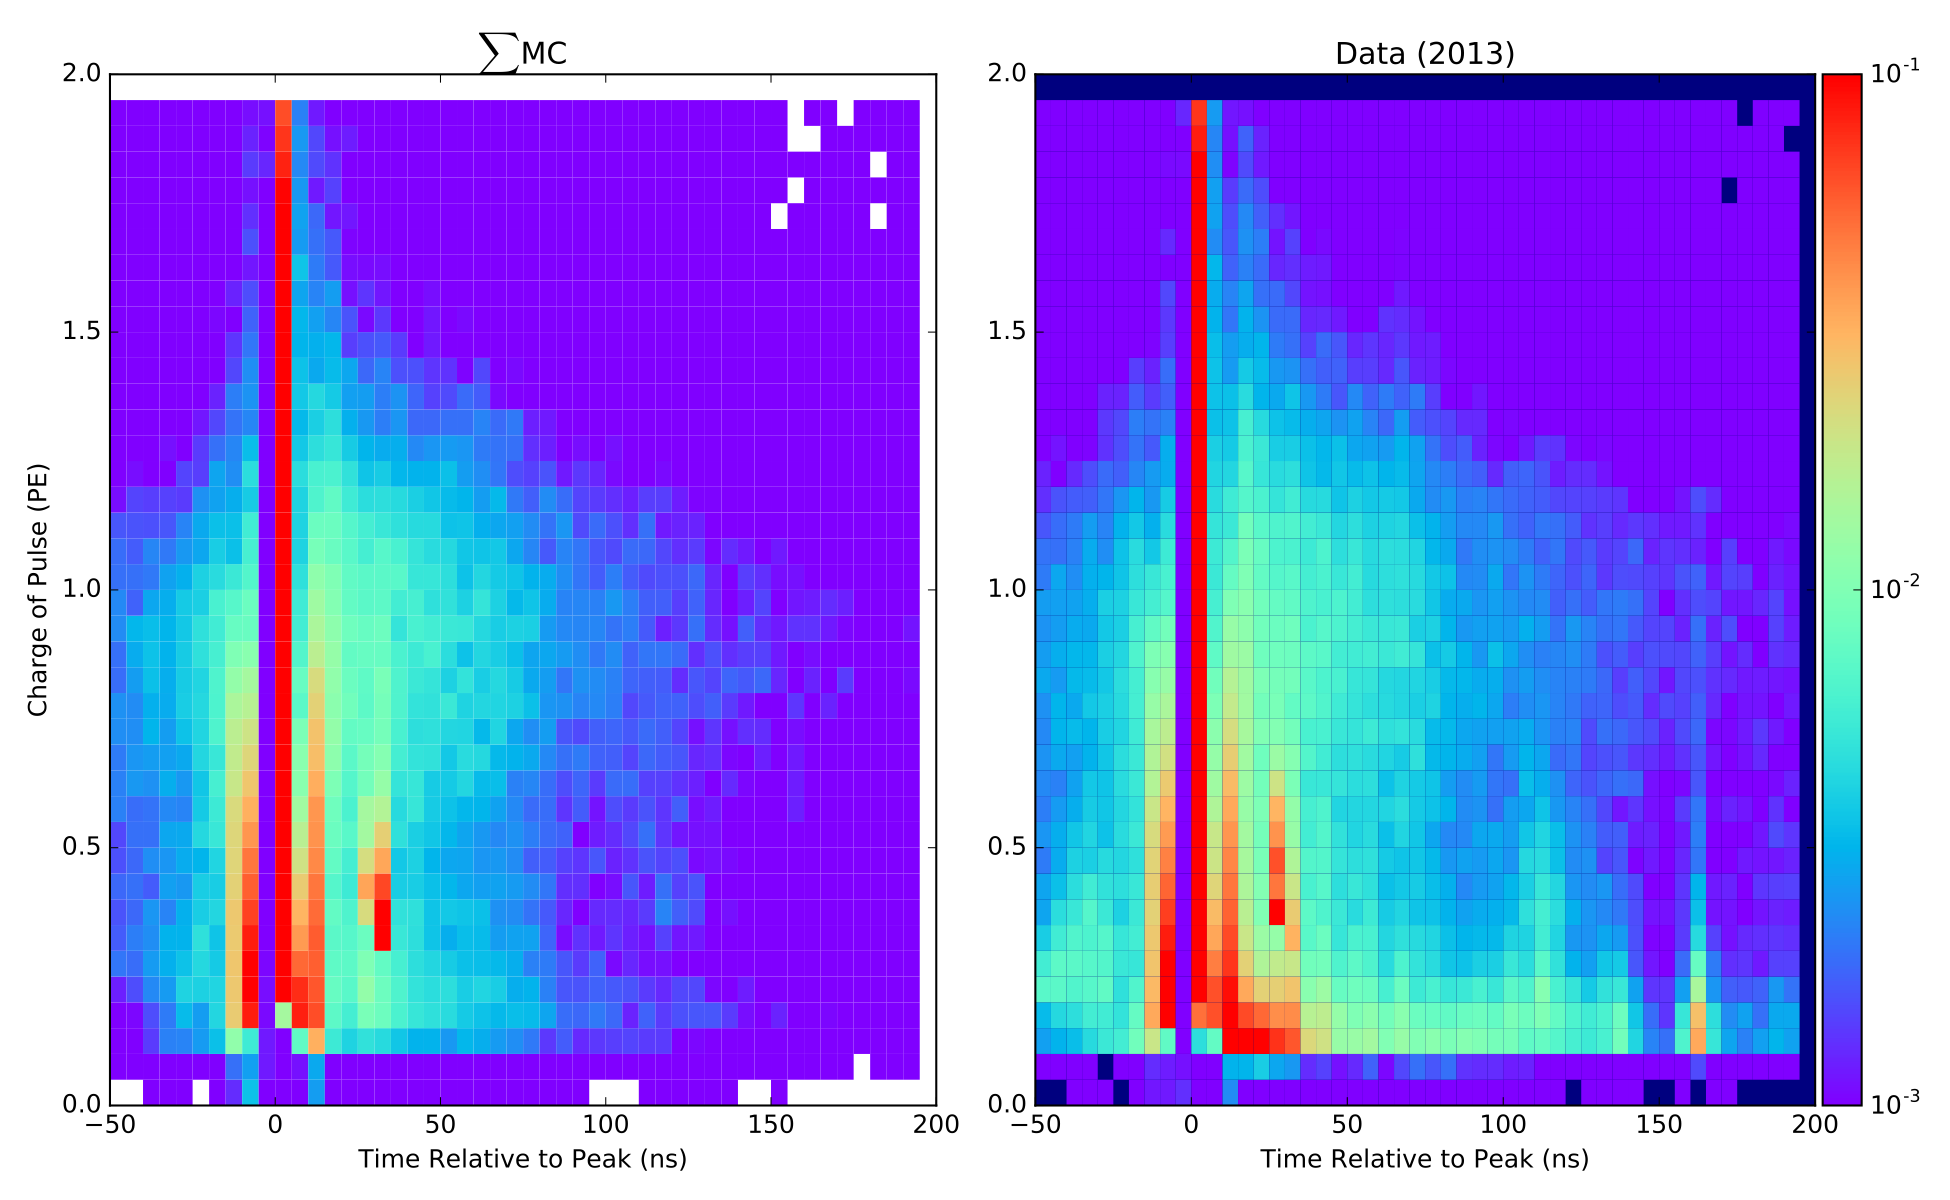
\includegraphics[width=0.9\linewidth]{2d_maps_detail_raw.png}
\caption{A comparison of the charge extraction in data and simulation at GRECO L7. Both the time and charge are shown for individual pulses on all DOMs. The time is measured relative to the largest pulse observed on each DOM during an event. The data and simulation histograms are independently normalized to 1.0. While the two show broad agreement, notable differences occur at low charge.}
\label{fig:pulse_timing_profile}
\end{figure}

Potential mismodeling effects of the charge extraction were checked in Figure~\ref{fig:pulse_timing_profile}. 
In these figures, the charge of each pulse is shown as a function of the measured time of the pulse, which is normalized to the time of the largest extracted pulse in the DOM for each event.

The erroneously split pulses are visible in data as a low-charge tail from t=0~ns until t=50~ns.
In addition to this effect, however, many other regions of disagreement are visible.
In data, there appear to be a significant number of prepulses not visible in the simulation occuring between t=-50~ns and t=-20~ns.
The structure of the late pulses, appearing with approximately 0.4 PE of charge and at time t=30~ns also appears notably different between the data and simulation.
A final set of pulses, occuring at 160~ns, also appears to be unsimulated.
All of the unsimulated features occur with charges less than 0.5 PE, a region strongly affected by the recalibration of the SPE templates.

These features remain unexplained. 
These may be the result of improper calibration of the PMTs, an incorrect SPE template used for charge extraction, or completely unknown effects.

It is currently unclear of the impact of the unsimulated features in analyses.
Each feature occurs at low charge and is not expected to contribute a significant fraction of the total charge of an event.
This timing structure requires additional calibration resources to identify and better simulate, the scope of which is beyond this work.
Regardless, the presence of unsimulated features indicates that at least some charge information in the simulation is an unreliable model of the data.

Charge information is used at many levels of the GRECO selection.
In order to excise charge from the selection, more than half of the variables used in the selection would need to be updated.
Each of these charge-related variables individually shows reasonable agreement between data and simulation.

In light of the existing agreement between data and simulation, and without a firm timescale for the correction and reproduction of new Monte Carlo sets, the decision was made to move forward with the GRECO analysis without changes to earlier cuts.
At Level 7, the observed disagreements in the pulses and the SPE templates led to the removal of charge information from the Pegleg reconstruction.


\subsection{Discovery of Flaring DOMs}
\label{subsec:flaring_doms}
Uncertainties in the ice model can lead to significant disagreements between data and simulation.
The existing uncertainties on the bulk ice assume that the coefficients for all ice layers are fully correlated.
However, it is possible that the ice model coefficients in parts of the detector are more poorly modeled than others.
By looking at the event rate in data and simulation as a function of the depth and position in the detector, discrepancies in the ice model may be identified.

\begin{figure}
\centering
	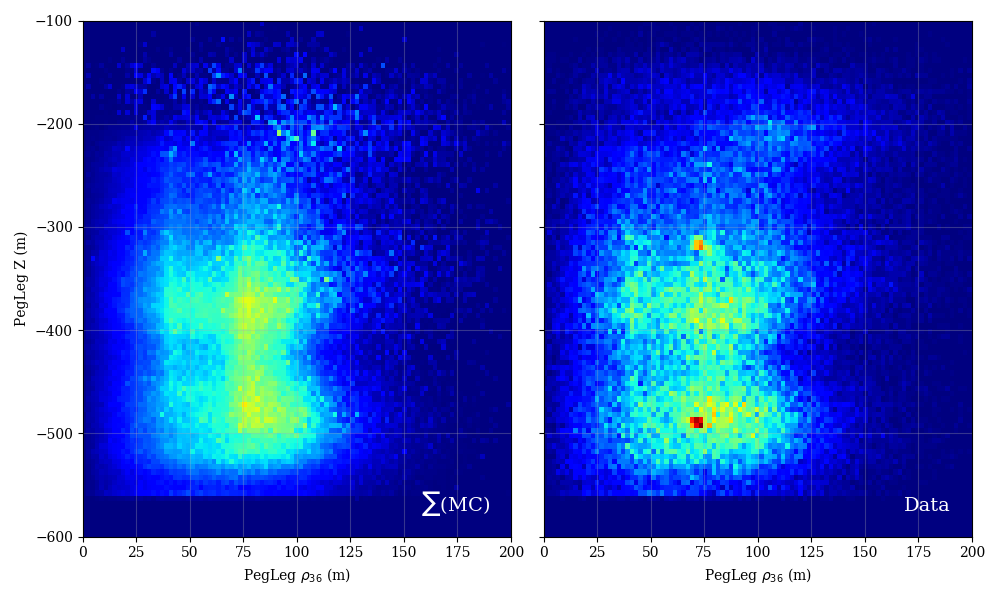
\includegraphics[width=0.9\linewidth]{pegleg_fine_z_rho.png}
\caption{The reconstructed Z position plotted against the reconstructed distance from string 36. The L7 cuts from GRECO have been removed for this plot. The colorbars in both plots have been normalized to be identical. The data and simulation show good agreement except for two points in the data, near ${\rho_{36}=75}$ at depths of -310 and -490. }
\label{fig:flaring_zrho}
\end{figure}

\begin{figure}
\centering
	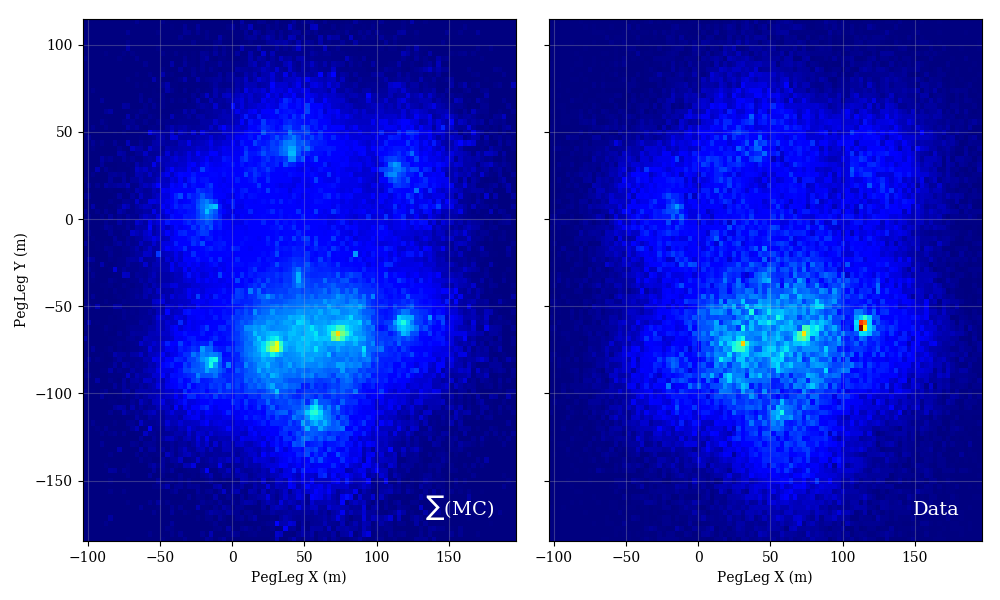
\includegraphics[width=0.9\linewidth]{pegleg_fine_x_y.png}
\caption{The reconstructed X position and Y position of events in the detector. The L7 cuts from GRECO have been removed for this plot. The colorbars in both plots have been normalized to be identical. Once again, reasonable agreement is observed in most regions, although data events have a clear excess near x=110 m, y=-60 m. This position corresponds to string 83.}
\label{fig:flaring_xy}
\end{figure}

Two-dimensional histograms of the depth and radial distance also show systematic disagreement in some regions, as shown in Figure~\ref{fig:flaring_zrho}.
These excess events appear to occur on a single string, string 83, shown in Figure~\ref{fig:flaring_xy}, indicating an effect occuring due to the DOM hardware in the detector.

Follow-up work has shown that these DOMs, known here as \emph{flaring DOMs}, appear to spontaneously emit light for unknown reasons. 
The light output is identifiable both based on the position of the hits and the amount of charge observed in nearby DOMs.
These spurious events, first discovered in the GRECO selection, have since spawned dedicated searches to better understand spontaneous light emission from the DOMs.
A small handful of DOMs have been identified by these searches with emission times as frequent as 1 Hz.

The affected events may be identified based on the charge profiles. 
DOMs directly adjacent to the emitting DOM observe a significant fraction of the total charge of the event.
This may be characterized using the 'charge RMS' of the event

\label{eqn:charge_rms}
\begin{equation}
	q_{RMS} = \frac{\sigma_q}{\sum_{hits}{q_i}}
\end{equation}

\begin{figure}
\centering
	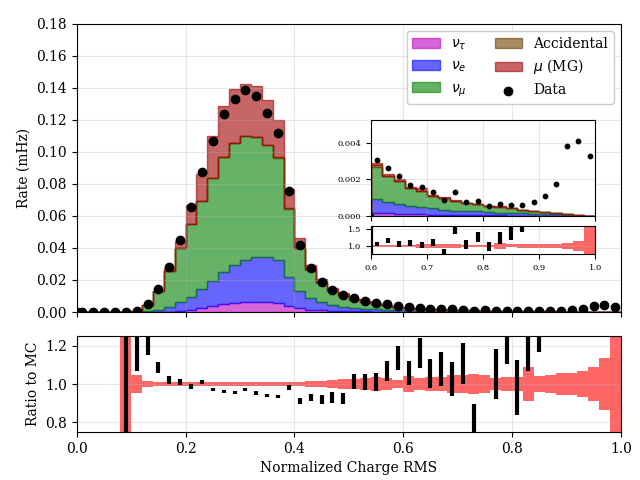
\includegraphics[width=0.9\linewidth]{L7_charge_rms_normalized.png}
\caption[The RMS of the charges showing the events with flaring DOMs]{The RMS of the charges within each event at Final Level. The value of the RMS is normalized using the total charge observed. The events with flaring DOMs cluster at high values of the charge RMS, visible in the inset.}
\label{fig:charge_rms}
\end{figure}

This is shown in Figure~\ref{fig:charge_rms}.
Events with a ${q_{RMS}}>0.85$ are cut from the analysis, removing the most obvious spurious events. 
A total of 975 events are removed from the GRECO data, resulting in a total reduction of 1.3\% of the event sample.
The removal of these events in data and simulation does not significantly impact the sample due to the low event rates involved.

\subsection{Simulation of Bedrock}
\label{subsec:bedrock}
Further investigations of the reconstructed Z position from Pegleg uncovered disagreements, shown in Figure~\ref{fig:reco_z}.
A small deficit of events in data is observed at ${Z\approx -450}$.
Checks performed with other samples have shown similar disagreeements at these depths, indicating disagreement in the ice model.
Previously unblinded oscillation samples showing this issue have not observed significant issues in the goodness-of-fit.
New ice models are underway with dedicated work to fix this region is underway.

\begin{figure}
\centering
	\includegraphics[width=0.9\linewidth]{L7_reco_z.png}
\caption{The reconstructed Z position using Pegleg. The GRECO L7 cuts have not been applied in order to show discrepancies below the detector. Noticeable disagreement is seen below the detector at a depth of -500~m. Additional disagreements are also visible at the top of DeepCore, a region dominated by atmospheric muons.}
\label{fig:reco_z}
\end{figure}

Near the bottom of the detector, a clear excess of events in data indicated a mismodeling in the simulation.
Events which interact below the detector typically require higher energies than those inside the fiducial volume in order to trigger DeepCore.

In the GRECO selection, events with energies above 1~TeV are modeled using NuGen simulation in order to account for events not properly simulated in the GENIE generator.
Previous investigations have shown that the two generators use similar models of the cross-section and return similar event rates at low levels.
The events from the NuGen generator were shown to make up a significant fraction of the high energy tail in the GRECO sample.
These events were therefore checked for potential issues.

The NuGen and GENIE simulated event samples are merged in the GRECO analyses after removing NuGen events in overlapping energy ranges.
The generated samples do include these overlapping regions, however.
For the purposes of testing, the full sample of GENIE and NuGen events were compared in true and reconstucted energy and Z position.
A comparison of the overlapping energy range of NuGen and GENIE events contained within the DeepCore fiducial volume showed some disagreement in the muon neutrino event sample.
Figure~\ref{fig:bedrock_energy} shows no disagreement in the neutral current and electron neutrino charged current events, indicating an effect specific to the muon neutrinos.

\begin{figure}
\centering
\includegraphics[width=0.9\linewidth]{log_true_energy.pdf}
\caption[The NuGen and GENIE true energy spectra at Final Level]{The NuGen and GENIE true energy spectra at Final Level. The neutrinos are shown without oscillations applied. The overlapping energy range, 100-1000~GeV, show good agreement between the two generators for neutral current and electron neutrino charged current interactions. The muon neutrinos disagree in the overlapping energy range. }
\label{fig:bedrock_energy}
\end{figure}

Limiting the energy raange of both samples to the overlapping region 100-1000 GeV, other distributions may be checked.
The cause of the discrepancy between the generators is shown in Figure~\ref{fig:bedrock_z}.
The two generators show broad agreement until a depth of approximately -830~m, corresponding to the interface between the Antarctic glacier and the underlying bedrock.
In the GRECO selection, only events with an outgoing muon have the range necessary to reach DeepCore from the bedrock.

\begin{figure}
\centering
\includegraphics[width=0.9\linewidth]{bedrock.pdf}
\caption[The NuGen and GENIE interaction depths at Final Level]{The NuGen and GENIE interaction depths at Final Level. Only events from the overlapping region of 100~GeV to 1~TeV are included. NuGen and GENIE agree above -830~m. The implementation of the GENIE generator in IceCube does not correctly model the bedrock at Z<-830~m.}
\label{fig:bedrock_z}
\end{figure}

Further checks discovered the issue in IceCube's implementation of the GENIE generator.
When calculating the interaction probability for the neutrino interactions, the density of material is included.
In the implementation of GENIE previously used by the IceCube collaboration, events were assumed to occur solely within or near the fiducial volume of DeepCore due to the low energies involved.
The bedrock was therefore deemed unnecessary and not implmented in favor of assuming a uniform density of ice throughout the simulation volume.
During initial implementation, the GENIE generator was planned for use up to 100~GeV due to technical limitations. 
Later work expanded this range up to 1~TeV with future work ongoing to push toward 10~TeV.
The problems with the bedrock were mistakenly overlooked during the upgrades of the generator, leading to the systematic disagreement shown in Figure~\ref{fig:reco_z}.

The bedrock has been properly included in both the NuGen generator as well as the PROPOSAL module for propagating the charged leptons.
GENIE events therefore suffer solely from an incorrect interaction probability due to the discovered bug.

In order to limit other potential issues from the bedrock, the analysis space was restricted, removing events below the bottom of the detector (${Z_{reco}\leq-500}$).
This cut significantly reduces the size of the sample by reducing the high energy events included at Final Level. 
The additional cut has some impact on the expected sensitivity, but was deemed necessary to minimize the potential impact of systematics issues associated with the bedrock events.


\subsection{Anisotropy of DeepCore}
\label{sec:azimuth_disagreement}
The reconstructed zenith and energy are used in the search for appearance.
The azimuthal direction is not used for oscillation searches, but was checked for agreement.

\begin{figure}
\centering
\includegraphics[width=0.9\linewidth]{L7_reco_azimuth.pdf}
\caption[The reconstructed azimuthal direction from Pegleg]{The reconstructed azimuthal direction from the Pegleg reconstruction at GRECO Level 7. The data and simulation have been scaled to the same rate. A variation as a function of azimuthal angle is seen in both the simulated events and data, although the effect is stronger in data.}
\label{fig:reco_azimuth}
\end{figure}

As described in Section~\ref{sec:bulk_ice}, the anisotropy of the ice model can bias the propagation of light in the detector in the azimuthal direction.
This can result in azimuthally biased reconstructions.
The anisotropy is simulated using a direction and magnitude, both of which are used to model the effect throughout the detector.
The IceCube simulation assumes that the anisotropy is independent of depth.

The reconstructed azimuthal directions from Pegleg in the GRECO sample is shown in Figure~\ref{fig:reco_azimuth}.
Both data and the simulated events show sinusoidal variation as a function of azimuthal direction, a result of the anisotropy in the ice.
The effect in data is stronger than in simulation, indicating that the average anisotropy of the DeepCore fiducial region is stronger than assumed for DeepCore.

The observed azimuthal disagreement of GRECO are the first hint that the anisotropy of the ice may not be uniform throughout the detector volume.
New calibration measurements to incorporate these new properties into the simulation are underway.
Because the anisotropy is not expected to directly impact the oscillation analysis, no additional cuts are introduced to the sample.












\graphicspath{{chapters/greco/images/level7/}}
\section{The Properties of the GRECO Event Selection}
\label{sec:greco_properties}
\begin{figure}
\includegraphics[width=\linewidth]{rate_vs_level.pdf} 
\caption[GRECO rates at each cut level]{The rates at each cut level. The muon and accidental trigger rate drops from around 18 Hz after the DeepCoreFilter to less than 1 mHz at Final Level.}
\label{fig:event_rates}
\end{figure}

The completion of cuts yields the completed GRECO event selection.
The rates of each simulation sample and of data are shown numerically in Table~\ref{tab:event_rates} or graphically in Figure~\ref{fig:event_rates}.
Also included is the analysis binning as described in Section~\ref{subsec:binning} for reference.

The sample is dominated by atmospheric muon neutrinos. 
The major source of statistical uncertainty, shown in Table~\ref{tab:sim_stats}, is the atmospheric muons.

\begin{table}[]
\centering
\begin{tabular}{@{}lllllllll@{}}
\toprule
Type              & \multicolumn{3}{c}{IceCube Processing}     & \multicolumn{4}{c}{GRECO}             & Analysis         \\ 
                     & Any Filter   & DC Filter  & Low-en L3        & L4         & L5       & L6    & L7          & Binning \\ \midrule
CORSIKA        & 990598     & 9178      & 969.818           & 50.511  & 4.100  & 0.443 & 0.100   & 0.092            \\
MuonGun        & 60669       & 2982      & 442.493          & 33.562  & 3.022   & 0.315 & 0.080   & 0.07             \\
Accidentals    & 35855       & 8117      & 283.559           & 11.963  & 1.799  & 0.102 & 0.002   & 0.001            \\
$\nu_e$        & 1.842        & 1.721     & 1.262               & 0.783    & 0.544  & 0.362 & 0.325   & 0.194            \\
$\nu_{\mu}$ & 11.317      & 6.360     & 4.758               & 2.503    & 1.629  & 1.011 & 0.676   & 0.552            \\
$\nu_{\tau}$ & 0.293        & 0.270     & 0.206              & 0.134    & 0.103  & 0.074 & 0.051   & 0.045            \\ \midrule
MC Total*       & 1026466   & 17303    & 1260               & 65.893  & 8.176  & 1.991 & 1.153   & 0.884            \\
Data              & 1154426   & 19092    & 1092               & 68.592   & 7.422  & 1.841 & 0.871   & 0.715            \\ \bottomrule
\end{tabular}
\caption{The event rates at each cut level in the GRECO selection. Note that the MuonGun events are included in this table, but do not contribute to the total Monte Carlo expectation to prevent double-counting of muon events from the CORSIKA sample. All rates are given in millihertz.}
\label{tab:event_rates}
\end{table}

\begin{table}[]
\centering
\begin{tabular}{@{}llll@{}}
\toprule
            & Simulated Events & Weighted Rate (Events) &  Uncertainty (Events) \\ \midrule
$\nu_e$     & 333892           & 12708                          & 26                   \\
$\nu_\mu$   & 842386           & 36134                          & 45                   \\
$\nu_\tau$  & 122765           & 2970                           & 13                   \\
MuonGun     & 2486             & 4651                           & 102                  \\
Accidentals & 12               & 85                             & 25                   \\ \bottomrule
\end{tabular}
\caption[Simulation uncertainties at GRECO Level 7]{The statistical uncertainties at GRECO Final Level. The sample is dominated by neutrinos, but the largest contributions to the statistical uncertainty are due to limited statistics in MuonGun and accidental triggers. The event rates are scaled to the appoximate number of events in data with an effective livetime of 2.3 years. }
\label{tab:sim_stats}
\end{table}

\subsection{Selecting Runs from Data}
\label{subsec:good_run_list}
Runs were selected from data to be used in the search for tau neutrino appearance based on four criteria:

\begin{description}
\item [InIce OK] Runs must not contain light from LEDs or other calibration devices
\item [All Strings] All 86 strings must have been taking data
\item [All DOMs] At least 5030 DOMs must be active during the entire run
\item [Full Runs] The run must be between 7 and 9 hours long. 
\end{description}

These conditions were used to identify "good" runs between May 2012 and April of 2015
A total of 968 days of detector data were selected resulting in 62406 events.

\subsection{Energy and Zenith Reach}
\label{subsubsec:greco_truth}
The GRECO sample covers a wide range of energies, with some Final Level events possessing energies as low as 2~GeV or as high as 1 TeV.
The bulk of the neutrino sample, shown in \ref{fig:true_nuproperties}, occurs at the expected oscillation minimum near 25 GeV.
Most neutrino events originate at the horizon, as expected from the atmospheric neutrino flux, although there exists an asymmetry between the upward- and downward-going events.
This asymmetry originates from the event selection, which selects against downward-going events in order to minimize the atmospheric muon background.

\begin{figure}[h]
\centering
\begin{tabular}[b]{c}
  \includegraphics[width=0.45\linewidth]{L7_true_coszen.png} \\
  \small (\textbf{\color{ctcolormain}a}) True Cos(Zenith)
\end{tabular} \hspace{2pt}
\begin{tabular}[b]{c}
  \includegraphics[width=0.45\linewidth]{L7_true_logen.png} \\
  \small (\textbf{\color{ctcolormain}b}) True $\Log_{10}$ Energy
\end{tabular}
\caption[GRECO Final Level zenith and energy spectrum]{The true neutrino energy and zenith of the GRECO sample at Final Level. The sample shows an asymmetry between upgoing (${cos(\theta)<0}$) and downgoing (${cos(\theta)>0}$) event rates in the neutrinos due to selection bias. The sample has a long tail of events at both high and low energies. Using the NuFit 2.2 oscillation parameters and the flux model from Honda, the ${\nu_\tau}$ events are observed in the very upgoing region around ${10^{1.4}=25}$ GeV. }
\label{fig:true_nuproperties}
\end{figure}

\subsection{Reconstructed Variables}
\label{subsubsec:greco_reco}
The true variables of the neutrino distributions are not observables in most GRECO analyses.
All events are described using the reconstructed energies and zenith angles from the Pegleg reconstruction, shown in Figure~\ref{fig:reco_nuproperties}.
The ${\nu_\tau}$ sample reconstructs to slightly lower energies due to the loss in energy from the outgoing neutrino.
The sample, when compared to data, shows reasonable shape agreement in both energy and zenith, although systematic disagreements occur above 100 GeV.

\begin{figure}[h]
\centering
\begin{tabular}[b]{c}
  \includegraphics[width=0.45\linewidth]{L7_reco_coszen.png} \\
  \small (\textbf{\color{ctcolormain}a}) Reco Cos(Zenith)
\end{tabular} \hspace{2pt}
\begin{tabular}[b]{c}
  \includegraphics[width=0.45\linewidth]{L7_reco_logen.png} \\
  \small (\textbf{\color{ctcolormain}b}) Reco $\Log_{10}$ Energy
\end{tabular}
\caption{The reconstructed energy and zenith of the GRECO sample at Final Level. Events in data reconstruct to both relatively high energies (${E_{R}>100}$ GeV) and very low energies (${E_{R}\approx2}$ GeV). Using the NuFit 2.2 oscillation parameters and the flux model from Honda, the ${\nu_\tau}$ events are observed in the very upgoing region around ${10^1.4=25}$ GeV. }
\label{fig:reco_nuproperties}
\end{figure}

The resolutions of the sample in energy and zenith are shown in Figures~\ref{fig:en_resolutions} and \ref{fig:coszen_resolutions}. 
The energy is well-reconstructed using Pegleg.
The neutral current and tau neutrino events lose energy to outgoing neutrinos, resulting in less light deposition and lower reconstructed energies.

\begin{figure}
\centering
  \includegraphics[width=0.9\linewidth]{resolution_energy.pdf} \\
\caption[Reconstructed zenith resolutions]{The resolution of the Pegleg reconstructed zenith of the GRECO sample at Final Level. The shaded band of each plot shows the 1$\sigma$ range for each plot. 
The Pegleg reconstruction energy resolution as a function of true energy. Cascade energies are well-reconstructed by Pegleg in the energy range of GRECO. The muon track is assumed to be minimum ionizing when calculating the associated energy. This assumption does not hold at higher energies. }
\label{fig:en_resolutions}
\end{figure}

\begin{figure}
\centering
  \includegraphics[width=0.9\linewidth]{resolution_coszen.pdf} \\
\caption[Reconstructed zenith resolutions]{The resolution of the Pegleg reconstructed zenith of the GRECO sample at Final Level. The shaded band of each plot shows the 1$\sigma$ range for each plot. 
The reconstruction fits to within $\Delta\cos\theta$=0.15 on average with better reconstruction resolution in the track-like muon neutrino charged current interactions. }
\label{fig:coszen_resolutions}
\end{figure}


